\hypertarget{sec-special}{%
\chapter{Beyond Regression and Classification}\label{sec-special}}

\vspace{-15mm}\addtocontents{toc}{\textit{Raphael Sonabend, Patrick Schratz and Damir Pulatov}}

\textbf{Raphael Sonabend} \newline  \emph{Imperial College London}

\textbf{Patrick Schratz} \newline  \emph{Friedrich Schiller University
Jena}

\textbf{Damir Pulatov} \newline  \emph{University of Wyoming}
\newline \newline 

So far, this book has only considered two tasks. In
Chapter~\ref{sec-basics} we introduced deterministic regression as well
as deterministic and probabilistic single-label classification
(Table~\ref{tbl-alltasks}). But our infrastructure also works well for
many other tasks, some of which are available in extension packages
(Figure~\ref{fig-mlr3verse}) and some are available by creating
pipelines with
\href{https://mlr3pipelines.mlr-org.com}{\texttt{mlr3pipelines}}\index{\texttt{mlr3pipelines}}.
In this chapter, we will take you through just a subset of these new
tasks, focusing on the ones that have a stable API. As we work through
this chapter we will refer to the `building blocks' of
\href{https://mlr3.mlr-org.com}{\texttt{mlr3}}\index{\texttt{mlr3}},
this refers to the base classes that must be extended to create new
tasks, these are
\href{https://mlr3.mlr-org.com/reference/Prediction.html}{\texttt{Prediction}},
\href{https://mlr3.mlr-org.com/reference/Learner.html}{\texttt{Learner}},
\href{https://mlr3.mlr-org.com/reference/Measure.html}{\texttt{Measure}},
and \href{https://mlr3.mlr-org.com/reference/Task.html}{\texttt{Task}}.
Table~\ref{tbl-alltasks} summarizes available extension tasks, including
the package(s) they are implemented in and a brief description of the
task.

\hypertarget{tbl-alltasks}{}
\begin{longtable}[]{@{}
  >{\raggedright\arraybackslash}p{(\columnwidth - 4\tabcolsep) * \real{0.4000}}
  >{\raggedright\arraybackslash}p{(\columnwidth - 4\tabcolsep) * \real{0.2000}}
  >{\raggedright\arraybackslash}p{(\columnwidth - 4\tabcolsep) * \real{0.4000}}@{}}
\caption{\label{tbl-alltasks}Table of extension tasks that can be used
with \texttt{mlr3} infrastructure. As we have a growing community of
contributors, this list is far from exhaustive and many `experimental'
task implementations exist; this list just represents the tasks that
have a functioning interface.}\tabularnewline
\toprule\noalign{}
\begin{minipage}[b]{\linewidth}\raggedright
Task
\end{minipage} & \begin{minipage}[b]{\linewidth}\raggedright
Package
\end{minipage} & \begin{minipage}[b]{\linewidth}\raggedright
Description
\end{minipage} \\
\midrule\noalign{}
\endfirsthead
\toprule\noalign{}
\begin{minipage}[b]{\linewidth}\raggedright
Task
\end{minipage} & \begin{minipage}[b]{\linewidth}\raggedright
Package
\end{minipage} & \begin{minipage}[b]{\linewidth}\raggedright
Description
\end{minipage} \\
\midrule\noalign{}
\endhead
\bottomrule\noalign{}
\endlastfoot
Deterministic regression &
\href{https://mlr3.mlr-org.com}{\texttt{mlr3}}\index{\texttt{mlr3}} &
Point prediction of a continuous variable. \\
Deterministic single-label classification &
\href{https://mlr3.mlr-org.com}{\texttt{mlr3}}\index{\texttt{mlr3}} &
Prediction of a single class for each observation. \\
Probabilistic single-label classification &
\href{https://mlr3.mlr-org.com}{\texttt{mlr3}}\index{\texttt{mlr3}} &
Prediction of the probability of an observation falling into one or more
mutually exclusive categories. \\
Cost-sensitive classification &
\href{https://mlr3.mlr-org.com}{\texttt{mlr3}}\index{\texttt{mlr3}} and
\href{https://mlr3pipelines.mlr-org.com}{\texttt{mlr3pipelines}}\index{\texttt{mlr3pipelines}}
& Classification predictions with unequal costs associated with
misclassifications. \\
Survival analysis &
\href{https://mlr3proba.mlr-org.com}{\texttt{mlr3proba}}\index{\texttt{mlr3proba}}
& Time-to-event predictions with possible `censoring'. \\
Density estimation &
\href{https://mlr3proba.mlr-org.com}{\texttt{mlr3proba}}\index{\texttt{mlr3proba}}
& Unsupervised estimation of probability density functions. \\
Spatiotemporal analysis &
\href{https://mlr3spatiotempcv.mlr-org.com}{\texttt{mlr3spatiotempcv}}\index{\texttt{mlr3spatiotempcv}}
and
\href{https://mlr3spatial.mlr-org.com}{\texttt{mlr3spatial}}\index{\texttt{mlr3spatial}}
& Supervised prediction of data with spatial (e.g., coordinates) and/or
temporal outcomes. \\
Cluster analysis &
\href{https://mlr3cluster.mlr-org.com}{\texttt{mlr3cluster}}\index{\texttt{mlr3cluster}}
& Unsupervised estimation of homogeneous clusters of data points. \\
\end{longtable}

\hypertarget{sec-cost-sens}{%
\section{Cost-Sensitive Classification}\label{sec-cost-sens}}

We begin by discussing a task that does not require any additional
packages or infrastructure, only the tools we have already learned about
from earlier chapters. In `regular' classification, the aim is to
optimize a metric (often the misclassification rate) while assuming all
misclassification errors are deemed equally severe. A more general
approach is cost-sensitive
classification\index{classification!cost-sensitive}{\marginnote{\begin{footnotesize}Cost-sensitive
Classification\end{footnotesize}}}, in which costs caused by different
kinds of errors may not be equal. The objective of cost-sensitive
classification is to minimize the expected costs. We will use
\texttt{tsk("german\_credit")} as a running example.

Imagine you are trying to calculate if giving someone a loan of \$5K
will result in a profit after one year, assuming they are expected to
pay back \$6K. To make this calculation, you will need to predict if the
person will have good credit. This is a deterministic classification
problem where we are predicting whether someone will be in class `Good'
or `Bad'. Now let us consider some potential costs associated with each
prediction and the eventual truth. As cost-sensitive classification is a
minimization problem, we assume lower costs correspond to higher
profits/positive outcomes, hence we write profits as negative values and
losses as positive values:

\begin{Shaded}
\begin{Highlighting}[]
\NormalTok{costs }\OtherTok{=} \FunctionTok{matrix}\NormalTok{(}\FunctionTok{c}\NormalTok{(}\SpecialCharTok{{-}}\DecValTok{1}\NormalTok{, }\DecValTok{0}\NormalTok{, }\DecValTok{5}\NormalTok{, }\DecValTok{0}\NormalTok{), }\AttributeTok{nrow =} \DecValTok{2}\NormalTok{, }\AttributeTok{dimnames =}
  \FunctionTok{list}\NormalTok{(}\StringTok{"Predicted Credit"} \OtherTok{=} \FunctionTok{c}\NormalTok{(}\StringTok{"good"}\NormalTok{, }\StringTok{"bad"}\NormalTok{),}
    \AttributeTok{Truth =} \FunctionTok{c}\NormalTok{(}\StringTok{"good"}\NormalTok{, }\StringTok{"bad"}\NormalTok{)))}
\NormalTok{costs}
\end{Highlighting}
\end{Shaded}

\begin{verbatim}
                Truth
Predicted Credit good bad
            good   -1   5
            bad     0   0
\end{verbatim}

In this example, if the model predicts that the individual has bad
credit (bottom row) then there is no profit or loss, the loan is not
provided. If the model predicts that the individual has good credit and
indeed the customer repays the loan with interest (top left), then you
will make a \$1K profit. On the other hand, if they default (top right),
you will lose \$5K.

\hypertarget{cost-sensitive-measure}{%
\subsection{Cost-Sensitive Measure}\label{cost-sensitive-measure}}

We will now see how to implement a more nuanced approach to
classification errors with \texttt{msr("classif.costs")}. This measure
takes one argument, which is a matrix with row and column names
corresponding to the class labels in the task of interest. Let us put
our insurance example into practice, notice that we have already named
the cost matrix as required for the measure:

\begin{Shaded}
\begin{Highlighting}[]
\FunctionTok{library}\NormalTok{(mlr3verse)}

\NormalTok{tsk\_german }\OtherTok{=} \FunctionTok{tsk}\NormalTok{(}\StringTok{"german\_credit"}\NormalTok{)}

\NormalTok{msr\_costs }\OtherTok{=} \FunctionTok{msr}\NormalTok{(}\StringTok{"classif.costs"}\NormalTok{, }\AttributeTok{costs =}\NormalTok{ costs)}
\NormalTok{msr\_costs}
\end{Highlighting}
\end{Shaded}

\begin{verbatim}
<MeasureClassifCosts:classif.costs>: Cost-sensitive Classification
* Packages: mlr3
* Range: [-Inf, Inf]
* Minimize: TRUE
* Average: macro
* Parameters: normalize=TRUE
* Properties: -
* Predict type: response
\end{verbatim}

\begin{Shaded}
\begin{Highlighting}[]
\NormalTok{learners }\OtherTok{=} \FunctionTok{lrns}\NormalTok{(}\FunctionTok{c}\NormalTok{(}\StringTok{"classif.log\_reg"}\NormalTok{, }\StringTok{"classif.featureless"}\NormalTok{,}
  \StringTok{"classif.ranger"}\NormalTok{))}
\NormalTok{bmr }\OtherTok{=} \FunctionTok{benchmark}\NormalTok{(}\FunctionTok{benchmark\_grid}\NormalTok{(tsk\_german, learners,}
  \FunctionTok{rsmp}\NormalTok{(}\StringTok{"cv"}\NormalTok{, }\AttributeTok{folds =} \DecValTok{3}\NormalTok{)))}
\NormalTok{bmr}\SpecialCharTok{$}\FunctionTok{aggregate}\NormalTok{(msr\_costs)[, }\FunctionTok{c}\NormalTok{(}\DecValTok{4}\NormalTok{, }\DecValTok{7}\NormalTok{)]}
\end{Highlighting}
\end{Shaded}

\begin{verbatim}
            learner_id classif.costs
1:     classif.log_reg        0.1791
2: classif.featureless        0.8002
3:      classif.ranger        0.2331
\end{verbatim}

In this experiment, we find that the logistic regression learner happens
to perform best as it minimizes the expected costs (and maximizes
expected profits) and the featureless learner performs the worst. All
losses result in positive costs, which means each model results in us
losing money. To improve our models, we will now turn to thresholding.

\hypertarget{thresholding-1}{%
\subsection{Thresholding}\label{thresholding-1}}

As we have discussed in Chapter~\ref{sec-basics},
thresholding\index{thresholding} is a method to fine-tune the
probability at which an observation will be predicted as one class label
or another. Currently in our running example, the models above will
predict a customer has good credit (in the class `Good') if the
probability of good credit is greater than 0.5. Here, this might not be
a sensible approach as we would likely act more conservatively and
reject more credit applications with a higher threshold due to the
non-uniform costs. This is highlighted in the \texttt{"threshold"}
\texttt{autoplot} (Figure~\ref{fig-costsens-threshold}), which plots
\texttt{msr("classif.costs")} over all possible thresholds.

\begin{Shaded}
\begin{Highlighting}[]
\NormalTok{prediction }\OtherTok{=} \FunctionTok{lrn}\NormalTok{(}\StringTok{"classif.log\_reg"}\NormalTok{,}
  \AttributeTok{predict\_type =} \StringTok{"prob"}\NormalTok{)}\SpecialCharTok{$}\FunctionTok{train}\NormalTok{(tsk\_german)}\SpecialCharTok{$}\FunctionTok{predict}\NormalTok{(tsk\_german)}
\FunctionTok{autoplot}\NormalTok{(prediction, }\AttributeTok{type =} \StringTok{"threshold"}\NormalTok{, }\AttributeTok{measure =}\NormalTok{ msr\_costs)}
\end{Highlighting}
\end{Shaded}

\begin{figure}

{\centering 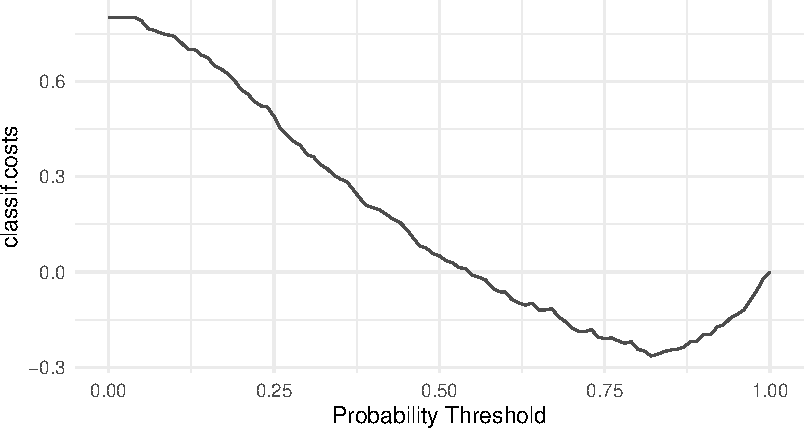
\includegraphics[width=1\textwidth,height=\textheight]{chapters/chapter13/beyond_regression_and_classification_files/figure-pdf/fig-costsens-threshold-1.pdf}

}

\caption{\label{fig-costsens-threshold}Changing values of cost-sensitive
measure as the prediction threshold is changed.}

\end{figure}

As expected, the optimal threshold is greater than 0.5 which means the
optimal model should predict `bad' credit more often than not.

The optimal threshold can be automated by making use of
\href{https://mlr3tuning.mlr-org.com}{\texttt{mlr3tuning}}\index{\texttt{mlr3tuning}}
(Chapter~\ref{sec-optimization}) and
\href{https://mlr3pipelines.mlr-org.com}{\texttt{mlr3pipelines}}\index{\texttt{mlr3pipelines}}
(Chapter~\ref{sec-pipelines}) to tune \texttt{po("tunethreshold")}.
Continuing the same example:

\begin{Shaded}
\begin{Highlighting}[]
\NormalTok{po\_cv }\OtherTok{=} \FunctionTok{po}\NormalTok{(}\StringTok{"learner\_cv"}\NormalTok{, }\FunctionTok{lrn}\NormalTok{(}\StringTok{"classif.log\_reg"}\NormalTok{, }\AttributeTok{predict\_type =} \StringTok{"prob"}\NormalTok{))}
\NormalTok{graph }\OtherTok{=}\NormalTok{  po\_cv }\SpecialCharTok{\%\textgreater{}\textgreater{}\%} \FunctionTok{po}\NormalTok{(}\StringTok{"tunethreshold"}\NormalTok{, }\AttributeTok{measure =}\NormalTok{ msr\_costs)}

\NormalTok{learners }\OtherTok{=} \FunctionTok{list}\NormalTok{(}\FunctionTok{as\_learner}\NormalTok{(graph), }\FunctionTok{lrn}\NormalTok{(}\StringTok{"classif.log\_reg"}\NormalTok{))}
\NormalTok{bmr }\OtherTok{=} \FunctionTok{benchmark}\NormalTok{(}\FunctionTok{benchmark\_grid}\NormalTok{(tsk\_german, learners,}
  \FunctionTok{rsmp}\NormalTok{(}\StringTok{"cv"}\NormalTok{, }\AttributeTok{folds =} \DecValTok{3}\NormalTok{)))}
\NormalTok{bmr}\SpecialCharTok{$}\FunctionTok{aggregate}\NormalTok{(msr\_costs)[, }\FunctionTok{c}\NormalTok{(}\DecValTok{4}\NormalTok{, }\DecValTok{7}\NormalTok{)]}
\end{Highlighting}
\end{Shaded}

\begin{verbatim}
                      learner_id classif.costs
1: classif.log_reg.tunethreshold       -0.1060
2:               classif.log_reg        0.1481
\end{verbatim}

By using \texttt{po("learner\_cv")} for internal resampling and
\texttt{po("tunethreshold")} to find the optimal threshold we have
improved our model performance considerably and can now even expect a
profit.

\hypertarget{sec-survival}{%
\section{Survival Analysis}\label{sec-survival}}

Survival analysis\index{survival analysis} is a field of statistics
concerned with trying to predict/estimate the time until an event takes
place. This predictive problem is unique as survival models are trained
and tested on data that may include `censoring', which occurs when the
event of interest does \emph{not} take place. Survival analysis can be
hard to explain in the abstract, so as a working example consider a
marathon runner in a race. Here the `survival problem' is trying to
predict the time when the marathon runner finishes the race. However, if
the event of interest does not take place (e.g., the marathon runner
gives up and does not finish the race), they are said to be censored.
Instead of throwing away information about censored events, survival
analysis datasets include a status variable that provides information
about the `status' of an observation. So in our example, we might write
the runner's outcome as \((4, 1)\) if they finish the race at four
hours, otherwise, if they give up at two hours we would write
\((2, 0)\).

The key to modeling in survival analysis is that we assume there exists
a hypothetical time the marathon runner would have finished if they had
not been censored, it is then the job of a survival learner to estimate
what the true survival time would have been for a similar runner,
assuming they are \emph{not} censored (see Figure~\ref{fig-censoring}).
Mathematically, this is represented by the hypothetical event time,
\(Y\), the hypothetical censoring time, \(C\), the observed outcome
time, \(T = \min(Y, C)\), the event indicator \(\Delta = (T = Y)\), and
as usual some features, \(X\). Learners are trained on \((T, \Delta)\)
but, critically, make predictions of \(Y\) from previously unseen
features. This means that unlike classification and regression, learners
are trained on two variables, \((T, \Delta)\), which, in R, is often
captured in a
\href{https://www.rdocumentation.org/packages/survival/topics/Surv}{\texttt{Surv}}
object. Relating to our example above, the runner's outcome would then
be \((T = 4, \Delta = 1)\) or \((T = 2, \Delta = 0)\). Another example
is in the code below, where we randomly generate six survival times and
six event indicators, an outcome with a \texttt{+} indicates the outcome
is censored, otherwise, the event of interest occurred.

\begin{Shaded}
\begin{Highlighting}[]
\FunctionTok{library}\NormalTok{(survival)}
\FunctionTok{Surv}\NormalTok{(}\FunctionTok{runif}\NormalTok{(}\DecValTok{6}\NormalTok{), }\FunctionTok{rbinom}\NormalTok{(}\DecValTok{6}\NormalTok{, }\DecValTok{1}\NormalTok{, }\FloatTok{0.5}\NormalTok{))}
\end{Highlighting}
\end{Shaded}

\begin{verbatim}
[1] 0.5523+ 0.2905  0.4404+ 0.1184  0.9216+ 0.7326 
\end{verbatim}

Readers familiar with survival analysis will recognize that the
description above applies specifically to `right censoring'. Currently,
this is the only form of censoring available in the \texttt{mlr3}
universe, hence restricting our discussion to that setting. For a good
introduction to survival analysis see Collett (2014) or for machine
learning in survival analysis specifically see R. Sonabend and Bender
(2023).

For the remainder of this section, we will look at how
\href{https://mlr3proba.mlr-org.com}{\texttt{mlr3proba}}\index{\texttt{mlr3proba}}
(R. Sonabend et al. 2021) extends the building blocks of \texttt{mlr3}
for survival analysis. We will begin by looking at objects used to
construct machine learning tasks for survival analysis, then we will
turn to the learners we have implemented to solve these tasks, before
looking at measures for evaluating survival analysis predictions, and
then finally we will consider how to transform prediction types.

\begin{figure}

{\centering 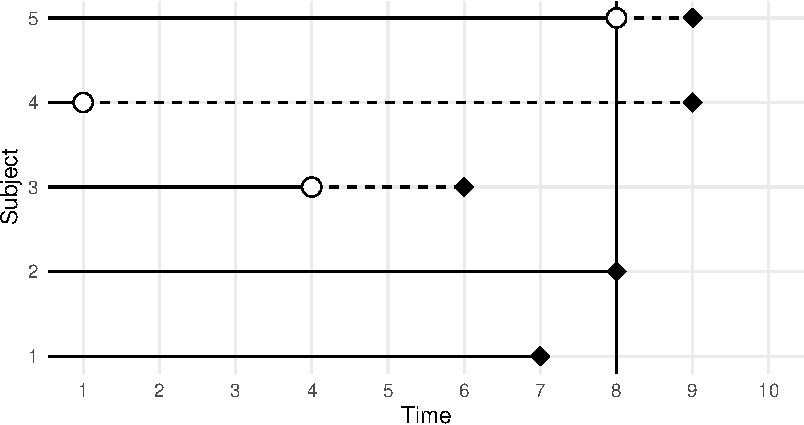
\includegraphics[width=1\textwidth,height=\textheight]{chapters/chapter13/beyond_regression_and_classification_files/figure-pdf/fig-censoring-1.pdf}

}

\caption{\label{fig-censoring}Plot illustrating different censoring
types. Dead and censored subjects (y-axis) over time (x-axis). Black
diamonds indicate true death times and white circles indicate censoring
times. Vertical line is the study end time. Subjects 1 and 2 die in the
study time. Subject 3 is censored in the study and (unknown) dies within
the study time. Subject 4 is censored in the study and (unknown) dies
after the study. Subject 5 dies after the end of the study. Figure and
caption from R. E. B. Sonabend (2021).}

\end{figure}

\hypertarget{tasksurv}{%
\subsection{TaskSurv}\label{tasksurv}}

As we saw in the introduction to this section, survival algorithms
require two targets for training, this means the new
\href{https://mlr3proba.mlr-org.com/reference/TaskSurv.html}{\texttt{TaskSurv}}
object expects two targets. The simplest way to create a survival task
is to use
\href{https://mlr3proba.mlr-org.com/reference/as_task_surv.html}{\texttt{as\_task\_surv()}},
as in the following code chunk. Note this has more arguments than
\href{https://mlr3.mlr-org.com/reference/as_task_regr.html}{\texttt{as\_task\_regr()}}
to reflect multiple target and censoring types, \texttt{time} and
\texttt{event} arguments expect strings representing column names where
the `time' and `event' variables are stored, \texttt{type} refers to the
censoring type (currently only right censoring supported so this is the
default). \texttt{as\_task\_surv()} coerces the target columns into a
\href{https://www.rdocumentation.org/packages/survival/topics/Surv}{\texttt{Surv}}
object. In this section we will use the \texttt{rats} dataset as a
running example, this dataset looks at predicting if a drug treatment
was successful in preventing 150 rats from developing tumors. The
dataset, by its own admission, is not perfect and should generally be
treated as `dummy' data, which is good for examples but not real-world
analysis.

\begin{Shaded}
\begin{Highlighting}[]
\FunctionTok{library}\NormalTok{(mlr3verse)}
\FunctionTok{library}\NormalTok{(mlr3proba)}
\FunctionTok{library}\NormalTok{(survival)}

\NormalTok{tsk\_rats }\OtherTok{=} \FunctionTok{as\_task\_surv}\NormalTok{(survival}\SpecialCharTok{::}\NormalTok{rats, }\AttributeTok{time =} \StringTok{"time"}\NormalTok{,}
  \AttributeTok{event =} \StringTok{"status"}\NormalTok{, }\AttributeTok{type =} \StringTok{"right"}\NormalTok{, }\AttributeTok{id =} \StringTok{"rats"}\NormalTok{)}

\NormalTok{tsk\_rats}\SpecialCharTok{$}\FunctionTok{head}\NormalTok{()}
\end{Highlighting}
\end{Shaded}

\begin{verbatim}
   time status litter rx sex
1:  101      0      1  1   f
2:   49      1      1  0   f
3:  104      0      1  0   f
4:   91      0      2  1   m
5:  104      0      2  0   m
6:  102      0      2  0   m
\end{verbatim}

Plotting the task with \texttt{autoplot} results in a
Kaplan-Meier\index{Kaplan-Meier} plot (Figure~\ref{fig-autokm}) which is
a non-parametric estimator of the probability of survival for the
average observation in the training set.

\begin{Shaded}
\begin{Highlighting}[]
\FunctionTok{autoplot}\NormalTok{(tsk\_rats)}
\end{Highlighting}
\end{Shaded}

\begin{figure}

{\centering 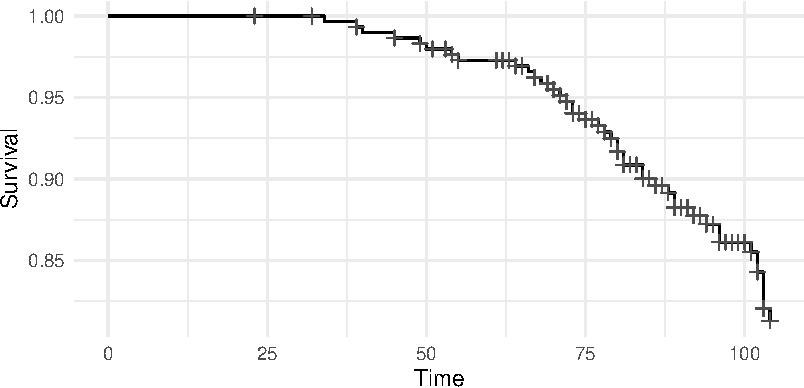
\includegraphics[width=1\textwidth,height=\textheight]{chapters/chapter13/beyond_regression_and_classification_files/figure-pdf/fig-autokm-1.pdf}

}

\caption{\label{fig-autokm}Kaplan-Meier plot of \texttt{tsk("rats")}.
x-axis is time variable and y-axis is survival function, S(T), defined
by \(1 -\) F(T) where F is the cumulative distribution function. Crosses
indicate points where censoring takes place.}

\end{figure}

As well as creating your own tasks, you can load any of the tasks
shipped with \texttt{mlr3proba}:

\begin{Shaded}
\begin{Highlighting}[]
\FunctionTok{as.data.table}\NormalTok{(mlr\_tasks)[task\_type }\SpecialCharTok{==} \StringTok{"surv"}\NormalTok{]}
\end{Highlighting}
\end{Shaded}

\begin{verbatim}
            key                  label task_type nrow ncol properties
1:         actg               ACTG 320      surv 1151   13           
2:         gbcs   German Breast Cancer      surv  686   10           
3:        grace             GRACE 1000      surv 1000    8           
4:         lung            Lung Cancer      surv  228   10           
5:         rats                   Rats      surv  300    5           
6: unemployment  Unemployment Duration      surv 3343    6           
7:         whas Worcester Heart Attack      surv  481   11           
7 variables not shown: [lgl, int, dbl, chr, fct, ord, pxc]
\end{verbatim}

\hypertarget{learnersurv-predictionsurv-and-predict-types}{%
\subsection{LearnerSurv, PredictionSurv and Predict
Types}\label{learnersurv-predictionsurv-and-predict-types}}

The interface for
\href{https://mlr3proba.mlr-org.com/reference/LearnerSurv.html}{\texttt{LearnerSurv}}
and
\href{https://mlr3proba.mlr-org.com/reference/PredictionSurv.html}{\texttt{PredictionSurv}}
objects is identical to the regression and classification settings
discussed in Chapter~\ref{sec-basics}. Similarly to these settings,
survival learners are constructed with
\href{https://mlr3.mlr-org.com/reference/mlr_sugar.html}{\texttt{lrn()}}.

\texttt{mlr3proba} has a different predict interface to \texttt{mlr3} as
all possible types of prediction (`predict types') are returned when
possible for all survival models -- i.e., if a model \emph{can} compute
a particular predict type then \emph{it will be} returned in
\texttt{PredictionSurv}. The reason for this design decision is that all
these predict types can be transformed to one another and it is
therefore computationally simpler to return all at once instead of
rerunning models to change predict type. In survival analysis, the
following predictions can be made:

\begin{itemize}
\tightlist
\item
  \texttt{response} -- Predicted survival time.
\item
  \texttt{distr} -- Predicted survival distribution, either discrete or
  continuous.
\item
  \texttt{lp} -- Linear predictor calculated as the fitted coefficients
  multiplied by the test data.
\item
  \texttt{crank} -- Continuous risk ranking.
\end{itemize}

We will go through each of these prediction types in more detail and
with examples to make them less abstract. We will use
\texttt{lrn("surv.coxph")}\index{Cox Proportional Hazards} trained on
\texttt{tsk("rats")} as a running example, for this model, all predict
types except \texttt{response} can be computed.

\begin{Shaded}
\begin{Highlighting}[]
\NormalTok{tsk\_rats }\OtherTok{=} \FunctionTok{tsk}\NormalTok{(}\StringTok{"rats"}\NormalTok{)}
\NormalTok{split }\OtherTok{=} \FunctionTok{partition}\NormalTok{(tsk\_rats)}
\NormalTok{prediction\_cph }\OtherTok{=} \FunctionTok{lrn}\NormalTok{(}\StringTok{"surv.coxph"}\NormalTok{)}\SpecialCharTok{$}\FunctionTok{train}\NormalTok{(tsk\_rats, split}\SpecialCharTok{$}\NormalTok{train)}\SpecialCharTok{$}
  \FunctionTok{predict}\NormalTok{(tsk\_rats, split}\SpecialCharTok{$}\NormalTok{test)}
\NormalTok{prediction\_cph}
\end{Highlighting}
\end{Shaded}

\begin{verbatim}
<PredictionSurv> for 99 observations:
    row_ids time status   crank      lp     distr
          8  102  FALSE -0.1577 -0.1577 <list[1]>
         16   98  FALSE -1.9549 -1.9549 <list[1]>
         24   76  FALSE -2.7150 -2.7150 <list[1]>
---                                              
        241   72   TRUE  0.8827  0.8827 <list[1]>
        247   73   TRUE  0.8897  0.8897 <list[1]>
        249   66   TRUE  0.1226  0.1226 <list[1]>
\end{verbatim}

\hypertarget{predict_type-response}{%
\subsubsection*{predict\_type =
``response''}\label{predict_type-response}}

Counterintuitively for many, the \texttt{response} prediction of
predicted survival times is the least common predict type in survival
analysis. The likely reason for this is due to the presence of
censoring. We rarely observe the true survival time for many
observations and therefore it is unlikely any survival model can
confidently make predictions for survival times. This is illustrated in
the code below.

In the example below we train and predict from a survival
SVM\index{support vector machine!survival} (\texttt{lrn("surv.svm")}),
note we use \texttt{type\ =\ "regression"} to select the algorithm that
optimizes survival time predictions and \texttt{gamma.mu\ =\ 1e-3} is
selected arbitrarily as this is a required parameter (this parameter
should usually be tuned). We then compare the predictions from the model
to the true data.

\begin{Shaded}
\begin{Highlighting}[]
\FunctionTok{library}\NormalTok{(mlr3extralearners)}
\NormalTok{prediction\_svm }\OtherTok{=} \FunctionTok{lrn}\NormalTok{(}\StringTok{"surv.svm"}\NormalTok{, }\AttributeTok{type =} \StringTok{"regression"}\NormalTok{, }\AttributeTok{gamma.mu =} \FloatTok{1e{-}3}\NormalTok{)}\SpecialCharTok{$}
  \FunctionTok{train}\NormalTok{(tsk\_rats, split}\SpecialCharTok{$}\NormalTok{train)}\SpecialCharTok{$}\FunctionTok{predict}\NormalTok{(tsk\_rats, split}\SpecialCharTok{$}\NormalTok{test)}
\FunctionTok{data.frame}\NormalTok{(}\AttributeTok{pred =}\NormalTok{ prediction\_svm}\SpecialCharTok{$}\NormalTok{response[}\DecValTok{1}\SpecialCharTok{:}\DecValTok{3}\NormalTok{],}
  \AttributeTok{truth =}\NormalTok{ prediction\_svm}\SpecialCharTok{$}\NormalTok{truth[}\DecValTok{1}\SpecialCharTok{:}\DecValTok{3}\NormalTok{])}
\end{Highlighting}
\end{Shaded}

\begin{verbatim}
   pred truth
1 88.19  102+
2 87.60   98+
3 87.21   76+
\end{verbatim}

As can be seen from the output, our predictions are all less than the
true observed time, which means we know our model underestimated the
truth. However, because each of the true values are censored times, we
have absolutely no way of knowing if these predictions are slightly bad
or absolutely terrible, (i.e., the true survival times could be
\(105, 99, 92\) or they could be \(300, 1000, 200\)). Hence, with no
realistic way to evaluate these models, survival time predictions are
rarely useful.

\hypertarget{predict_type-distr}{%
\subsubsection*{predict\_type = ``distr''}\label{predict_type-distr}}

Unlike regression in which deterministic/point predictions are most
common, in survival analysis distribution predictions are much more
common. You will therefore find that the majority of survival models in
\texttt{mlr3proba} will make distribution predictions by default. These
predictions are implemented using the
\href{https://alan-turing-institute.r-universe.dev/ui\#package:distr6}{\texttt{distr6}}
package, which allows visualization and evaluation of survival curves
(defined as \(1 -\) cumulative distribution function). Below we extract
the first three \texttt{\$distr} predictions from our running example
and calculate the probability of survival at \(t = 77\).

\begin{Shaded}
\begin{Highlighting}[]
\NormalTok{prediction\_cph}\SpecialCharTok{$}\NormalTok{distr[}\DecValTok{1}\SpecialCharTok{:}\DecValTok{3}\NormalTok{]}\SpecialCharTok{$}\FunctionTok{survival}\NormalTok{(}\DecValTok{77}\NormalTok{)}
\end{Highlighting}
\end{Shaded}

\begin{verbatim}
     [,1]   [,2]   [,3]
77 0.9213 0.9865 0.9937
\end{verbatim}

The output indicates that there is a 92.1\%, 98.7\%, 99.4\%, chance of
the first three predicted rats being alive at time 77 respectively.

\hypertarget{predict_type-lp}{%
\subsubsection*{predict\_type = ``lp''}\label{predict_type-lp}}

\texttt{lp}, often written as \(\eta\) in academic writing, is
computationally the simplest prediction and has a natural analog in
regression modeling. Readers familiar with linear regression will know
that when fitting a simple linear regression model, \(Y = X\beta\), we
are estimating the values for \(\beta\), and the estimated linear
predictor\index{linear predictor} (lp) is then \(X\hat{\beta}\), where
\(\hat{\beta}\) are our estimated coefficients. In simple survival
models, the linear predictor is the same quantity (but estimated in a
slightly more complicated way). The learner implementations in
\texttt{mlr3proba} are primarily machine-learning focused and few of
these models have a simple linear form, which means that \texttt{lp}
cannot be computed for most of these. In practice, when used for
prediction, \texttt{lp} is a proxy for a relative risk/continuous
ranking prediction, which is discussed next.

\hypertarget{predict_type-crank}{%
\subsubsection*{predict\_type = ``crank''}\label{predict_type-crank}}

The final prediction type, \texttt{crank}, is the most common in
survival analysis and perhaps also the most confusing. Academic texts
will often refer to `risk' predictions in survival analysis (hence why
survival models are often known as `risk prediction models'), without
defining what `risk' means. Often, risk is defined as \(\exp(\eta)\) as
this is a common quantity found in simple linear survival models.
However, sometimes risk is defined as \(\exp(-\eta)\), and sometimes it
can be an arbitrary quantity that does not have a meaningful
interpretation. To prevent this confusion in \texttt{mlr3proba}, we
define the predict type \texttt{crank}, which stands for
\textbf{c}ontinuous \textbf{rank}ing. This is best explained by example;
continuing from the previous we output the first three \texttt{crank}
predictions.

\begin{Shaded}
\begin{Highlighting}[]
\NormalTok{prediction\_cph}\SpecialCharTok{$}\NormalTok{crank[}\DecValTok{1}\SpecialCharTok{:}\DecValTok{3}\NormalTok{]}
\end{Highlighting}
\end{Shaded}

\begin{verbatim}
      1       2       3 
-0.1577 -1.9549 -2.7150 
\end{verbatim}

The output tells us that the first rat is at the lowest risk of death
(smaller values represent lower risk) and the third rat is at the
highest risk. The distance between predictions also tells us that the
difference in risk between the second and third rats is smaller than the
difference between the first and second. The actual values themselves
are meaningless and therefore comparing \texttt{crank} values between
samples (or papers or experiments) is not meaningful.

The \texttt{crank} prediction type is informative and common in practice
because it allows identifying observations at lower/higher risk to each
other, which is useful for resource allocation, e.g., which patient
should be given an expensive treatment, and clinical trials, e.g., are
people in a treatment arm at lower risk of disease X than people in the
control arm.

\begin{tcolorbox}[enhanced jigsaw, opacitybacktitle=0.6, rightrule=.15mm, opacityback=0, arc=.35mm, breakable, titlerule=0mm, colframe=quarto-callout-warning-color-frame, coltitle=black, bottomrule=.15mm, toprule=.15mm, colback=white, colbacktitle=quarto-callout-warning-color!10!white, bottomtitle=1mm, toptitle=1mm, title=\textcolor{quarto-callout-warning-color}{\faExclamationTriangle}\hspace{0.5em}{Interpreting Survival Risk}, leftrule=.75mm, left=2mm]

The interpretation of `risk' for survival predictions differs across R
packages and sometimes even between models in the same package. In
\texttt{mlr3proba} there is one consistent interpretation of
\texttt{crank}: lower values represent a lower risk of the event taking
place and higher values represent higher risk.

\end{tcolorbox}

\hypertarget{measuresurv}{%
\subsection{MeasureSurv}\label{measuresurv}}

Survival models in \texttt{mlr3proba} are evaluated with
\href{https://mlr3proba.mlr-org.com/reference/MeasureSurv.html}{\texttt{MeasureSurv}}
objects, which are constructed in the usual way with \texttt{msr()}.

In general survival measures can be grouped into the following:

\begin{enumerate}
\def\labelenumi{\arabic{enumi}.}
\tightlist
\item
  Discrimination measures -- Quantify if a model correctly identifies if
  one observation is at higher risk than another. Evaluate
  \texttt{crank} and/or \texttt{lp} predictions.
\item
  Calibration measures -- Quantify if the average prediction is close to
  the truth (all definitions of calibration are unfortunately vague in a
  survival context). Evaluate \texttt{crank} and/or \texttt{distr}
  predictions.
\item
  Scoring rules -- Quantify if probabilistic predictions are close to
  true values. Evaluate \texttt{distr} predictions.
\end{enumerate}

\begin{Shaded}
\begin{Highlighting}[]
\FunctionTok{as.data.table}\NormalTok{(mlr\_measures)[}
\NormalTok{  task\_type }\SpecialCharTok{==} \StringTok{"surv"}\NormalTok{, }\FunctionTok{c}\NormalTok{(}\StringTok{"key"}\NormalTok{, }\StringTok{"predict\_type"}\NormalTok{)][}\DecValTok{1}\SpecialCharTok{:}\DecValTok{5}\NormalTok{]}
\end{Highlighting}
\end{Shaded}

\begin{verbatim}
                  key predict_type
1:         surv.brier        distr
2:   surv.calib_alpha        distr
3:    surv.calib_beta           lp
4: surv.chambless_auc           lp
5:        surv.cindex        crank
\end{verbatim}

There is not a consensus in the literature around the `best' survival
measures to use to evaluate models. We recommend RCLL (right-censored
logloss) (\texttt{msr("surv.rcll")}) to evaluate the quality of
\texttt{distr} predictions, concordance index
(\texttt{msr("surv.cindex")}) to evaluate a model's discrimination, and
D-Calibration (\texttt{msr("surv.dcalib")}) to evaluate a model's
calibration.

Using these measures, we can now evaluate our predictions from the
previous example.

\begin{Shaded}
\begin{Highlighting}[]
\NormalTok{prediction\_cph}\SpecialCharTok{$}\FunctionTok{score}\NormalTok{(}\FunctionTok{msrs}\NormalTok{(}\FunctionTok{c}\NormalTok{(}\StringTok{"surv.rcll"}\NormalTok{, }\StringTok{"surv.cindex"}\NormalTok{, }\StringTok{"surv.dcalib"}\NormalTok{)))}
\end{Highlighting}
\end{Shaded}

\begin{verbatim}
  surv.rcll surv.cindex surv.dcalib 
     4.0879      0.8593      0.7463 
\end{verbatim}

The model's performance seems okay as the RCLL and DCalib are relatively
low 0 and the C-index is greater than 0.5 however it is very hard to
determine the performance of any survival model without comparing it to
some baseline (usually the Kaplan-Meier).

\hypertarget{sec-surv-comp}{%
\subsection{Composition}\label{sec-surv-comp}}

Throughout \texttt{mlr3proba} documentation we refer to ``native'' and
``composed'' predictions. We define a `native' prediction as the
prediction made by a model without any post-processing, whereas a
`composed' prediction is returned after post-processing.

\hypertarget{internal-composition}{%
\subsubsection{Internal Composition}\label{internal-composition}}

\texttt{mlr3proba} makes use of composition internally to return a
\texttt{"crank"} prediction for every learner. This is to ensure that we
can meaningfully benchmark all models according to at least one
criterion. The package uses the following rules to create
\texttt{"crank"} predictions:

\begin{enumerate}
\def\labelenumi{\arabic{enumi}.}
\tightlist
\item
  If a model returns a `risk' prediction then \texttt{crank\ =\ risk}
  (we may multiply this by \(-1\) to ensure the `low-value low-risk'
  interpretation).
\item
  Else if a model returns a \texttt{response} prediction then we set
  \texttt{crank\ =\ -response}.
\item
  Else if a model returns a \texttt{lp} prediction then we set
  \texttt{crank\ =\ lp} (or \texttt{crank\ =\ -lp} if needed).
\item
  Else if a model returns a \texttt{distr} prediction then we set
  \texttt{crank} as the sum of the cumulative hazard function (see R.
  Sonabend, Bender, and Vollmer (2022) for full discussion as to why we
  picked this method).
\end{enumerate}

\hypertarget{explicit-composition-and-pipelines}{%
\subsubsection{Explicit Composition and
Pipelines}\label{explicit-composition-and-pipelines}}

At the start of this section, we mentioned that it is possible to
transform prediction types between each other. In \texttt{mlr3proba}
this is possible with `compositor' pipelines
(Chapter~\ref{sec-pipelines}). There are several pipelines implemented
in the package but two in particular focus on predict type
transformation:

\begin{enumerate}
\def\labelenumi{\arabic{enumi}.}
\tightlist
\item
  \href{https://mlr3proba.mlr-org.com/reference/mlr_graphs_crankcompositor.html}{\texttt{pipeline\_crankcompositor()}}
  -- Transforms a \texttt{"distr"} prediction to \texttt{"crank"}
\item
  \href{https://mlr3proba.mlr-org.com/reference/mlr_graphs_distrcompositor.html}{\texttt{pipeline\_distrcompositor()}}
  -- Transforms a \texttt{"lp"} prediction to \texttt{"distr"}
\end{enumerate}

In practice, the second pipeline is more common as we internally use a
version of the first pipeline whenever we return predictions from
survival models (so only use the first pipeline to overwrite these
ranking predictions), and so we will just look at the second pipeline.

In the example below we load the \texttt{rats} dataset, remove factor
columns, and then partition the data into training and testing. We
construct the \texttt{distrcompositor} pipeline around a survival GLMnet
learner (\texttt{lrn("surv.glmnet")}) which by default can only make
predictions for \texttt{"lp"} and \texttt{"crank"}. In the pipeline, we
specify that we will estimate the baseline distribution with a
Kaplan-Meier\index{Kaplan-Meier} estimator
(\texttt{estimator\ =\ "kaplan"}) and that we want to assume a
proportional hazards form for our estimated distribution
(\texttt{form\ =\ "ph"}). We then train and predict in the usual way and
in our output we can now see a \texttt{distr} prediction.

\begin{Shaded}
\begin{Highlighting}[]
\FunctionTok{library}\NormalTok{(mlr3verse)}
\FunctionTok{library}\NormalTok{(mlr3extralearners)}

\NormalTok{tsk\_rats }\OtherTok{=} \FunctionTok{tsk}\NormalTok{(}\StringTok{"rats"}\NormalTok{)}\SpecialCharTok{$}\FunctionTok{select}\NormalTok{(}\FunctionTok{c}\NormalTok{(}\StringTok{"litter"}\NormalTok{, }\StringTok{"rx"}\NormalTok{))}
\NormalTok{split }\OtherTok{=} \FunctionTok{partition}\NormalTok{(tsk\_rats)}

\NormalTok{learner }\OtherTok{=} \FunctionTok{lrn}\NormalTok{(}\StringTok{"surv.glmnet"}\NormalTok{)}

\CommentTok{\# no distr output}
\NormalTok{learner}\SpecialCharTok{$}\FunctionTok{train}\NormalTok{(tsk\_rats, split}\SpecialCharTok{$}\NormalTok{train)}\SpecialCharTok{$}\FunctionTok{predict}\NormalTok{(tsk\_rats, split}\SpecialCharTok{$}\NormalTok{test)}
\end{Highlighting}
\end{Shaded}

\begin{verbatim}
<PredictionSurv> for 99 observations:
    row_ids time status crank.1   lp.1
          9  104  FALSE  0.0249 0.0249
         10   91  FALSE  0.7997 0.7997
         15  104  FALSE  0.0415 0.0415
---                                   
        236   81   TRUE  0.6558 0.6558
        249   66   TRUE  0.6890 0.6890
        289  103   TRUE  1.5717 1.5717
\end{verbatim}

\begin{Shaded}
\begin{Highlighting}[]
\NormalTok{graph\_learner }\OtherTok{=} \FunctionTok{as\_learner}\NormalTok{(}\FunctionTok{ppl}\NormalTok{(}
  \StringTok{"distrcompositor"}\NormalTok{,}
  \AttributeTok{learner =}\NormalTok{ learner,}
  \AttributeTok{estimator =} \StringTok{"kaplan"}\NormalTok{,}
  \AttributeTok{form =} \StringTok{"ph"}
\NormalTok{))}

\CommentTok{\# now with distr}
\NormalTok{graph\_learner}\SpecialCharTok{$}\FunctionTok{train}\NormalTok{(tsk\_rats, split}\SpecialCharTok{$}\NormalTok{train)}\SpecialCharTok{$}\FunctionTok{predict}\NormalTok{(tsk\_rats, split}\SpecialCharTok{$}\NormalTok{test)}
\end{Highlighting}
\end{Shaded}

\begin{verbatim}
<PredictionSurv> for 99 observations:
    row_ids time status crank.1   lp.1     distr
          9  104  FALSE  0.0249 0.0249 <list[1]>
         10   91  FALSE  0.7997 0.7997 <list[1]>
         15  104  FALSE  0.0415 0.0415 <list[1]>
---                                             
        236   81   TRUE  0.6558 0.6558 <list[1]>
        249   66   TRUE  0.6890 0.6890 <list[1]>
        289  103   TRUE  1.5717 1.5717 <list[1]>
\end{verbatim}

Mathematically, we have done the following:

\begin{enumerate}
\def\labelenumi{\arabic{enumi}.}
\tightlist
\item
  Assume our estimated distribution will have the form
  \(h(t) = h_0(t)\exp(\eta)\) where \(h\) is the hazard function and
  \(h_0\) is the baseline hazard function.
\item
  Estimate \(\hat{\eta}\) prediction using GLMnet
\item
  Estimate \(\hat{h}_0(t)\) with the Kaplan-Meier estimator
\item
  Put this all together as \(h(t) = \hat{h}_0(t)\exp(\hat{\eta})\)
\end{enumerate}

For more detail about prediction types and composition we recommend
Kalbfleisch and Prentice (2011).

\hypertarget{sec-survival-all}{%
\subsection{Putting It All Together}\label{sec-survival-all}}

Finally, we will put all the above into practice in a small benchmark
experiment. We first load \texttt{tsk("grace")} (which only has numeric
features) and sample 500 rows randomly. We then select the RCLL,
D-Calibration, and C-index to evaluate predictions, set up the same
pipeline we used in the previous experiment, and load a Cox PH and
Kaplan-Meier estimator. We run our experiment with three-fold CV and
aggregate the results.

\begin{Shaded}
\begin{Highlighting}[]
\FunctionTok{library}\NormalTok{(mlr3extralearners)}

\NormalTok{tsk\_grace }\OtherTok{=} \FunctionTok{tsk}\NormalTok{(}\StringTok{"grace"}\NormalTok{)}
\NormalTok{tsk\_grace}\SpecialCharTok{$}\FunctionTok{filter}\NormalTok{(}\FunctionTok{sample}\NormalTok{(tsk\_grace}\SpecialCharTok{$}\NormalTok{nrow, }\DecValTok{500}\NormalTok{))}
\NormalTok{msr\_txt }\OtherTok{=} \FunctionTok{c}\NormalTok{(}\StringTok{"surv.rcll"}\NormalTok{, }\StringTok{"surv.cindex"}\NormalTok{, }\StringTok{"surv.dcalib"}\NormalTok{)}
\NormalTok{measures }\OtherTok{=} \FunctionTok{msrs}\NormalTok{(msr\_txt)}

\NormalTok{graph\_learner }\OtherTok{=} \FunctionTok{as\_learner}\NormalTok{(}\FunctionTok{ppl}\NormalTok{(}
  \StringTok{"distrcompositor"}\NormalTok{,}
  \AttributeTok{learner =} \FunctionTok{lrn}\NormalTok{(}\StringTok{"surv.glmnet"}\NormalTok{),}
  \AttributeTok{estimator =} \StringTok{"kaplan"}\NormalTok{,}
  \AttributeTok{form =} \StringTok{"ph"}
\NormalTok{))}
\NormalTok{graph\_learner}\SpecialCharTok{$}\NormalTok{id }\OtherTok{=} \StringTok{"Coxnet"}
\NormalTok{learners }\OtherTok{=} \FunctionTok{c}\NormalTok{(}\FunctionTok{lrns}\NormalTok{(}\FunctionTok{c}\NormalTok{(}\StringTok{"surv.coxph"}\NormalTok{, }\StringTok{"surv.kaplan"}\NormalTok{)), graph\_learner)}

\NormalTok{bmr }\OtherTok{=} \FunctionTok{benchmark}\NormalTok{(}\FunctionTok{benchmark\_grid}\NormalTok{(tsk\_grace, learners,}
  \FunctionTok{rsmp}\NormalTok{(}\StringTok{"cv"}\NormalTok{, }\AttributeTok{folds =} \DecValTok{3}\NormalTok{)))}
\NormalTok{bmr}\SpecialCharTok{$}\FunctionTok{aggregate}\NormalTok{(measures)[, }\FunctionTok{c}\NormalTok{(}\StringTok{"learner\_id"}\NormalTok{, ..msr\_txt)]}
\end{Highlighting}
\end{Shaded}

\begin{verbatim}
    learner_id surv.rcll surv.cindex surv.dcalib
1:  surv.coxph     5.220      0.8250       5.050
2: surv.kaplan     5.438      0.5000       4.152
3:      Coxnet     5.212      0.8264      12.164
\end{verbatim}

In this small experiment, Coxnet and Cox PH have the best
discrimination, the Kaplan-Meier baseline has the best calibration, and
Coxnet and Cox PH have similar overall predictive accuracy (with the
lowest RCLL).

\hypertarget{sec-density}{%
\section{Density Estimation}\label{sec-density}}

Density estimation\index{density estimation} is a learning task to
estimate the unknown distribution from which a univariate dataset is
generated or put more simply to estimate the probability density (or
mass) function for a single variable. As with survival analysis, density
estimation is implemented in \texttt{mlr3proba}, as both can make
probability distribution predictions (hence the name
``\textbf{mlr3proba}bilistic''). Unconditional density estimation
(i.e.~estimation of a target without any covariates) is viewed as an
unsupervised task, which means the `truth' is never known. For a good
overview of density estimation see Silverman (1986).

The package \texttt{mlr3proba} extends \texttt{mlr3} with the following
objects for density estimation:

\begin{itemize}
\tightlist
\item
  \href{https://mlr3proba.mlr-org.com/reference/TaskDens.html}{\texttt{TaskDens}}
  to define density tasks.
\item
  \href{https://mlr3proba.mlr-org.com/reference/LearnerDens.html}{\texttt{LearnerDens}}
  as the base class for density estimators.
\item
  \href{https://mlr3proba.mlr-org.com/reference/PredictionDens.html}{\texttt{PredictionDens}}
  for density predictions.
\item
  \href{https://mlr3proba.mlr-org.com/reference/MeasureDens.html}{\texttt{MeasureDens}}
  as a specialized class for density performance measures.
\end{itemize}

We will consider each in turn.

\hypertarget{taskdens}{%
\subsection{TaskDens}\label{taskdens}}

As density estimation is an unsupervised task, there is no target for
prediction. In the code below we construct a density task using
\href{https://mlr3proba.mlr-org.com/reference/as_task_dens.html}{\texttt{as\_task\_dens()}}
which takes one argument, a \texttt{data.frame} type object with exactly
one column (which we will use to estimate the underlying distribution).

\begin{Shaded}
\begin{Highlighting}[]
\NormalTok{tsk\_dens }\OtherTok{=} \FunctionTok{as\_task\_dens}\NormalTok{(}\FunctionTok{data.table}\NormalTok{(}\AttributeTok{x =} \FunctionTok{rnorm}\NormalTok{(}\DecValTok{1000}\NormalTok{)))}
\NormalTok{tsk\_dens}
\end{Highlighting}
\end{Shaded}

\begin{verbatim}
<TaskDens:data.table(x = rnorm(1000))> (1000 x 1)
* Target: -
* Properties: -
* Features (1):
  - dbl (1): x
\end{verbatim}

As with other tasks, we have included a couple of tasks that come
shipped with \texttt{mlr3proba}:

\begin{Shaded}
\begin{Highlighting}[]
\FunctionTok{as.data.table}\NormalTok{(mlr\_tasks)[task\_type }\SpecialCharTok{==} \StringTok{"dens"}\NormalTok{, }\FunctionTok{c}\NormalTok{(}\DecValTok{1}\SpecialCharTok{:}\DecValTok{2}\NormalTok{, }\DecValTok{4}\SpecialCharTok{:}\DecValTok{5}\NormalTok{)]}
\end{Highlighting}
\end{Shaded}

\begin{verbatim}
        key                  label nrow ncol
1: faithful Old Faithful Eruptions  272    1
2:   precip   Annual Precipitation   70    1
\end{verbatim}

\hypertarget{learnerdens-and-predictiondens}{%
\subsection{LearnerDens and
PredictionDens}\label{learnerdens-and-predictiondens}}

Density learners may return the following prediction types:

\begin{enumerate}
\def\labelenumi{\arabic{enumi}.}
\tightlist
\item
  \texttt{distr} -- probability distribution
\item
  \texttt{pdf} -- probability density function
\item
  \texttt{cdf} -- cumulative distribution function
\end{enumerate}

All learners will return a \texttt{distr} and \texttt{pdf} prediction
but only some can make \texttt{cdf} predictions. Again, the
\texttt{distr} predict type is implemented using \texttt{distr6}. In the
code below we train and `predict' with a histogram learner and then plot
the estimated probability density function (Figure~\ref{fig-dens-hist}),
which closely matches the underlying Normally-distributed data.

\begin{Shaded}
\begin{Highlighting}[]
\NormalTok{lrn\_hist }\OtherTok{=} \FunctionTok{lrn}\NormalTok{(}\StringTok{"dens.hist"}\NormalTok{)}
\NormalTok{prediction }\OtherTok{=}\NormalTok{ lrn\_hist}\SpecialCharTok{$}\FunctionTok{train}\NormalTok{(tsk\_dens, }\DecValTok{1}\SpecialCharTok{:}\DecValTok{900}\NormalTok{)}\SpecialCharTok{$}\FunctionTok{predict}\NormalTok{(tsk\_dens, }\DecValTok{901}\SpecialCharTok{:}\DecValTok{1000}\NormalTok{)}
\NormalTok{x }\OtherTok{=} \FunctionTok{seq.int}\NormalTok{(}\SpecialCharTok{{-}}\DecValTok{2}\NormalTok{, }\DecValTok{2}\NormalTok{, }\FloatTok{0.01}\NormalTok{)}
\NormalTok{df }\OtherTok{=} \FunctionTok{data.frame}\NormalTok{(}\AttributeTok{x =}\NormalTok{ x, }\AttributeTok{y =}\NormalTok{ prediction}\SpecialCharTok{$}\NormalTok{distr}\SpecialCharTok{$}\FunctionTok{pdf}\NormalTok{(x))}
\FunctionTok{ggplot}\NormalTok{(df, }\FunctionTok{aes}\NormalTok{(}\AttributeTok{x =}\NormalTok{ x, }\AttributeTok{y =}\NormalTok{ y)) }\SpecialCharTok{+} \FunctionTok{geom\_line}\NormalTok{() }\SpecialCharTok{+} \FunctionTok{theme\_minimal}\NormalTok{()}
\end{Highlighting}
\end{Shaded}

\begin{figure}[H]

{\centering 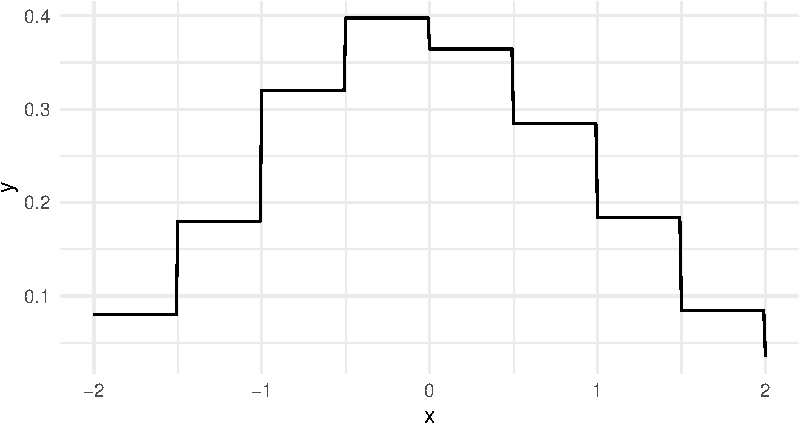
\includegraphics[width=1\textwidth,height=\textheight]{chapters/chapter13/beyond_regression_and_classification_files/figure-pdf/fig-dens-hist-1.pdf}

}

\caption{\label{fig-dens-hist}Predicted density from the histogram
learner, which closely resembles the underlying N(0, 1) data.}

\end{figure}

The \texttt{pdf} and \texttt{cdf} predict types are simply wrappers
around \texttt{distr\$pdf} and \texttt{distr\$cdf} respectively:

\begin{Shaded}
\begin{Highlighting}[]
\NormalTok{prediction }\OtherTok{=}\NormalTok{ lrn\_hist}\SpecialCharTok{$}\FunctionTok{train}\NormalTok{(tsk\_dens, }\DecValTok{1}\SpecialCharTok{:}\DecValTok{10}\NormalTok{)}\SpecialCharTok{$}\FunctionTok{predict}\NormalTok{(tsk\_dens, }\DecValTok{11}\SpecialCharTok{:}\DecValTok{13}\NormalTok{)}
\CommentTok{\# pdf and cdf columns in output}
\NormalTok{prediction}
\end{Highlighting}
\end{Shaded}

\begin{verbatim}
<PredictionDens> for 3 observations:
 row_ids pdf    cdf              distr
      11 0.4 0.1803 <Distribution[39]>
      12 0.0 0.0000 <Distribution[39]>
      13 0.2 0.9963 <Distribution[39]>
\end{verbatim}

\begin{Shaded}
\begin{Highlighting}[]
\CommentTok{\# comparing cdf from prediction to $cdf method from distr}
\FunctionTok{cbind}\NormalTok{(prediction}\SpecialCharTok{$}\NormalTok{distr}\SpecialCharTok{$}\FunctionTok{cdf}\NormalTok{(tsk\_dens}\SpecialCharTok{$}\FunctionTok{data}\NormalTok{()}\SpecialCharTok{$}\NormalTok{x[}\DecValTok{11}\SpecialCharTok{:}\DecValTok{13}\NormalTok{]),}
\NormalTok{  prediction}\SpecialCharTok{$}\NormalTok{cdf[}\DecValTok{1}\SpecialCharTok{:}\DecValTok{3}\NormalTok{])}
\end{Highlighting}
\end{Shaded}

\begin{verbatim}
       [,1]   [,2]
[1,] 0.1803 0.1803
[2,] 0.0000 0.0000
[3,] 0.9963 0.9963
\end{verbatim}

\hypertarget{measuredens-and-putting-it-all-together}{%
\subsection{MeasureDens and Putting It All
Together}\label{measuredens-and-putting-it-all-together}}

At the time of publication, the only measure implemented in
\texttt{mlr3proba} for density estimation is logloss, which is defined
in the same way as in classification, \(L(y) = -\log(\hat{f}_Y(y))\),
where \(\hat{f}_Y\) is our estimated probability density function.
Putting this together with the above we are now ready to train a density
learner, estimate a distribution, and evaluate our estimation:

\begin{Shaded}
\begin{Highlighting}[]
\NormalTok{msr\_logloss }\OtherTok{=} \FunctionTok{msr}\NormalTok{(}\StringTok{"dens.logloss"}\NormalTok{)}
\NormalTok{msr\_logloss}
\end{Highlighting}
\end{Shaded}

\begin{verbatim}
<MeasureDensLogloss:dens.logloss>: Log Loss
* Packages: mlr3, mlr3proba
* Range: [0, Inf]
* Minimize: TRUE
* Average: macro
* Parameters: eps=1e-15
* Properties: -
* Predict type: pdf
\end{verbatim}

\begin{Shaded}
\begin{Highlighting}[]
\NormalTok{prediction}\SpecialCharTok{$}\FunctionTok{score}\NormalTok{(msr\_logloss)}
\end{Highlighting}
\end{Shaded}

\begin{verbatim}
dens.logloss 
       12.35 
\end{verbatim}

This output is most easily interpreted when compared to other learners
in a benchmark experiment, so let us put everything together to conduct
a small benchmark study on \texttt{tsk("faithful")} task using some of
the integrated density learners:

\begin{Shaded}
\begin{Highlighting}[]
\FunctionTok{library}\NormalTok{(mlr3extralearners)}
\NormalTok{tsk\_faithful }\OtherTok{=} \FunctionTok{tsk}\NormalTok{(}\StringTok{"faithful"}\NormalTok{)}
\NormalTok{learners }\OtherTok{=} \FunctionTok{lrns}\NormalTok{(}\FunctionTok{c}\NormalTok{(}\StringTok{"dens.hist"}\NormalTok{, }\StringTok{"dens.pen"}\NormalTok{, }\StringTok{"dens.kde"}\NormalTok{))}
\NormalTok{measure }\OtherTok{=} \FunctionTok{msr}\NormalTok{(}\StringTok{"dens.logloss"}\NormalTok{)}
\NormalTok{bmr }\OtherTok{=} \FunctionTok{benchmark}\NormalTok{(}\FunctionTok{benchmark\_grid}\NormalTok{(tsk\_faithful, learners,}
  \FunctionTok{rsmp}\NormalTok{(}\StringTok{"cv"}\NormalTok{, }\AttributeTok{folds =} \DecValTok{3}\NormalTok{)))}
\NormalTok{bmr}\SpecialCharTok{$}\FunctionTok{aggregate}\NormalTok{(measure)}
\end{Highlighting}
\end{Shaded}

\begin{Shaded}
\begin{Highlighting}[]
\FunctionTok{autoplot}\NormalTok{(bmr, }\AttributeTok{measure =}\NormalTok{ measure)}
\end{Highlighting}
\end{Shaded}

\begin{figure}

{\centering 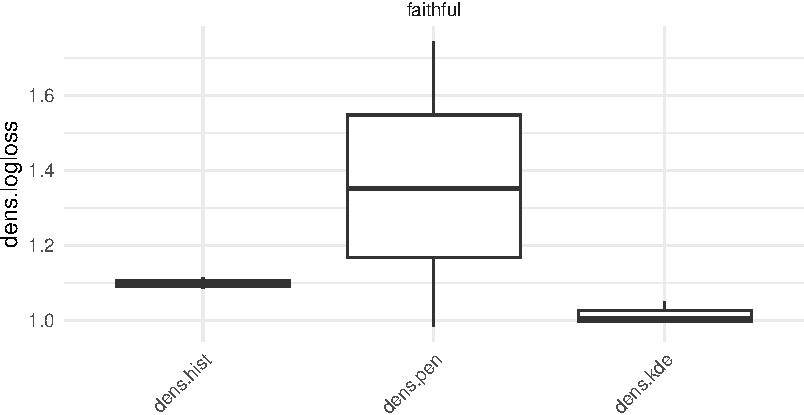
\includegraphics[width=1\textwidth,height=\textheight]{chapters/chapter13/beyond_regression_and_classification_files/figure-pdf/fig-beyond-density-1.pdf}

}

\caption{\label{fig-beyond-density}Three boxplots comparing performance
of dens.hist, dens.pen, and dens.kde on \texttt{tsk("faithful")}.}

\end{figure}

The results (Figure~\ref{fig-beyond-density}) of this experiment
indicate that the sophisticated Penalized Density Estimator does not
outperform the baseline histogram, but the Kernel Density Estimator has
at least consistently better (i.e.~lower) logloss results.

\hypertarget{sec-cluster}{%
\section{Cluster Analysis}\label{sec-cluster}}

Cluster analysis\index{cluster analysis} is another unsupervised task
implemented in \texttt{mlr3}. The objective of cluster analysis is to
group data into clusters, where each cluster contains similar
observations. The similarity is based on specified metrics that are task
and application-dependent. Unlike classification where we try to predict
a class for each observation, in cluster analysis there is no `true'
label or class to predict.

The package
\href{https://mlr3cluster.mlr-org.com}{\texttt{mlr3cluster}}\index{\texttt{mlr3cluster}}
extends \texttt{mlr3} with the following objects for cluster analysis:

\begin{itemize}
\tightlist
\item
  \href{https://mlr3cluster.mlr-org.com/reference/TaskClust.html}{\texttt{TaskClust}}
  to define clustering tasks
\item
  \href{https://mlr3cluster.mlr-org.com/reference/LearnerClust.html}{\texttt{LearnerClust}}
  as the base class for clustering learners
\item
  \href{https://mlr3cluster.mlr-org.com/reference/PredictionClust.html}{\texttt{PredictionClust}}
  as the specialized class for
  \href{https://mlr3.mlr-org.com/reference/Prediction.html}{\texttt{Prediction}}
  objects
\item
  \href{https://mlr3cluster.mlr-org.com/reference/MeasureClust.html}{\texttt{MeasureClust}}
  as the specialized class for performance measures
\end{itemize}

We will consider each in turn.

\hypertarget{taskclust}{%
\subsection{TaskClust}\label{taskclust}}

Similarly to density estimation (Section~\ref{sec-density}), there is no
target for prediction and so no \texttt{truth} field in
\href{https://mlr3cluster.mlr-org.com/reference/TaskClust.html}{\texttt{TaskClust}}.
By example, we will look at the
\href{https://www.rdocumentation.org/packages/cluster/topics/ruspini}{\texttt{ruspini}}
dataset, which has 75 rows and two columns and was first introduced in
Ruspini (1970) to illustrate different clustering techniques. The
observations in the dataset form four natural clusters
(Figure~\ref{fig-beyond-clust-ruspini}). In the code below we construct
a cluster task using
\href{https://mlr3cluster.mlr-org.com/reference/as_task_clust.html}{\texttt{as\_task\_clust()}}
which only takes one argument, a \texttt{data.frame} type object.

\begin{Shaded}
\begin{Highlighting}[]
\FunctionTok{library}\NormalTok{(mlr3verse)}
\FunctionTok{library}\NormalTok{(cluster)}
\NormalTok{tsk\_ruspini }\OtherTok{=} \FunctionTok{as\_task\_clust}\NormalTok{(ruspini)}
\NormalTok{tsk\_ruspini}
\end{Highlighting}
\end{Shaded}

\begin{verbatim}
<TaskClust:ruspini> (75 x 2)
* Target: -
* Properties: -
* Features (2):
  - int (2): x, y
\end{verbatim}

\begin{Shaded}
\begin{Highlighting}[]
\NormalTok{tsk\_ruspini}\SpecialCharTok{$}\FunctionTok{data}\NormalTok{(}\DecValTok{1}\SpecialCharTok{:}\DecValTok{3}\NormalTok{) }\CommentTok{\# print first 3 rows}
\end{Highlighting}
\end{Shaded}

\begin{verbatim}
    x  y
1:  4 53
2:  5 63
3: 10 59
\end{verbatim}

\begin{Shaded}
\begin{Highlighting}[]
\FunctionTok{autoplot}\NormalTok{(tsk\_ruspini)}
\end{Highlighting}
\end{Shaded}

\begin{figure}[H]

{\centering 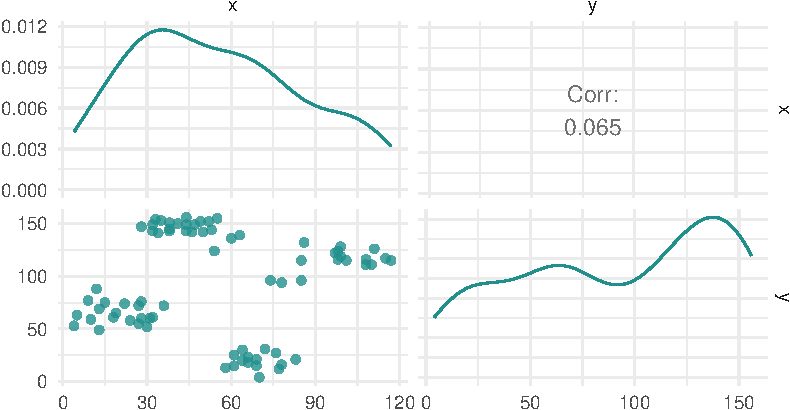
\includegraphics[width=1\textwidth,height=\textheight]{chapters/chapter13/beyond_regression_and_classification_files/figure-pdf/fig-beyond-clust-ruspini-1.pdf}

}

\caption{\label{fig-beyond-clust-ruspini}Distribution of the
\texttt{ruspini} dataset.}

\end{figure}

Technically, we did not need to create a new task for the
\texttt{ruspini} dataset since it is already included in the package,
along with one other task:

\begin{Shaded}
\begin{Highlighting}[]
\FunctionTok{as.data.table}\NormalTok{(mlr\_tasks)[task\_type }\SpecialCharTok{==} \StringTok{"clust"}\NormalTok{, }\FunctionTok{c}\NormalTok{(}\DecValTok{1}\SpecialCharTok{:}\DecValTok{2}\NormalTok{, }\DecValTok{4}\SpecialCharTok{:}\DecValTok{5}\NormalTok{)]}
\end{Highlighting}
\end{Shaded}

\begin{verbatim}
         key      label nrow ncol
1:   ruspini    Ruspini   75    2
2: usarrests US Arrests   50    4
\end{verbatim}

\hypertarget{learnerclust-and-predictionclust}{%
\subsection{LearnerClust and
PredictionClust}\label{learnerclust-and-predictionclust}}

As with density estimation, we refer to \texttt{training} and
\texttt{predicting} for clustering to be consistent with the
\texttt{mlr3} interface, but strictly speaking, this should be
\texttt{clustering} and \texttt{assigning} (the latter we will return to
shortly). Two \texttt{predict\_types} are available for clustering
learners:

\begin{enumerate}
\def\labelenumi{\arabic{enumi}.}
\tightlist
\item
  \texttt{"partition"} -- Estimate of which cluster an observation falls
  into
\item
  \texttt{"prob"} -- Probability of an observation belonging to each
  cluster
\end{enumerate}

Similarly to classification, prediction types of clustering learners are
either deterministic (\texttt{"partition"}) or probabilistic
(\texttt{"prob"}).

Below we construct a C-Means clustering learner with \texttt{"prob"}
prediction type and three clusters (\texttt{centers\ =\ 3}), train it on
the \texttt{ruspini} dataset and then return the cluster assignments
(\texttt{\$assignments}) for six random observations.

\begin{Shaded}
\begin{Highlighting}[]
\NormalTok{lrn\_cmeans }\OtherTok{=} \FunctionTok{lrn}\NormalTok{(}\StringTok{"clust.cmeans"}\NormalTok{, }\AttributeTok{predict\_type =} \StringTok{"prob"}\NormalTok{, }\AttributeTok{centers =} \DecValTok{3}\NormalTok{)}
\NormalTok{lrn\_cmeans}
\end{Highlighting}
\end{Shaded}

\begin{verbatim}
<LearnerClustCMeans:clust.cmeans>: Fuzzy C-Means Clustering Learner
* Model: -
* Parameters: centers=3
* Packages: mlr3, mlr3cluster, e1071
* Predict Types:  partition, [prob]
* Feature Types: logical, integer, numeric
* Properties: complete, fuzzy, partitional
\end{verbatim}

\begin{Shaded}
\begin{Highlighting}[]
\NormalTok{lrn\_cmeans}\SpecialCharTok{$}\FunctionTok{train}\NormalTok{(tsk\_ruspini)}
\NormalTok{lrn\_cmeans}\SpecialCharTok{$}\NormalTok{assignments[}\FunctionTok{sample}\NormalTok{(tsk\_ruspini}\SpecialCharTok{$}\NormalTok{nrow, }\DecValTok{6}\NormalTok{)]}
\end{Highlighting}
\end{Shaded}

\begin{verbatim}
[1] 1 2 1 3 1 3
\end{verbatim}

As clustering is unsupervised, it often does not make sense to use
\texttt{predict} for new data however this is still possible using the
\texttt{mlr3} interface.

\begin{Shaded}
\begin{Highlighting}[]
\CommentTok{\# using different data for estimation (rare use case)}
\NormalTok{lrn\_cmeans}\SpecialCharTok{$}\FunctionTok{train}\NormalTok{(tsk\_ruspini, }\DecValTok{1}\SpecialCharTok{:}\DecValTok{30}\NormalTok{)}\SpecialCharTok{$}\FunctionTok{predict}\NormalTok{(tsk\_ruspini, }\DecValTok{31}\SpecialCharTok{:}\DecValTok{32}\NormalTok{)}
\end{Highlighting}
\end{Shaded}

\begin{verbatim}
<PredictionClust> for 2 observations:
 row_ids partition prob.1  prob.2  prob.3
      31         1 0.9663 0.01815 0.01552
      32         1 0.9782 0.01178 0.01002
\end{verbatim}

\begin{Shaded}
\begin{Highlighting}[]
\CommentTok{\# using same data as for estimation (common use case)}
\NormalTok{prediction }\OtherTok{=}\NormalTok{ lrn\_cmeans}\SpecialCharTok{$}\FunctionTok{train}\NormalTok{(tsk\_ruspini)}\SpecialCharTok{$}\FunctionTok{predict}\NormalTok{(tsk\_ruspini)}
\FunctionTok{autoplot}\NormalTok{(prediction, tsk\_ruspini)}
\end{Highlighting}
\end{Shaded}

\begin{figure}[H]

{\centering 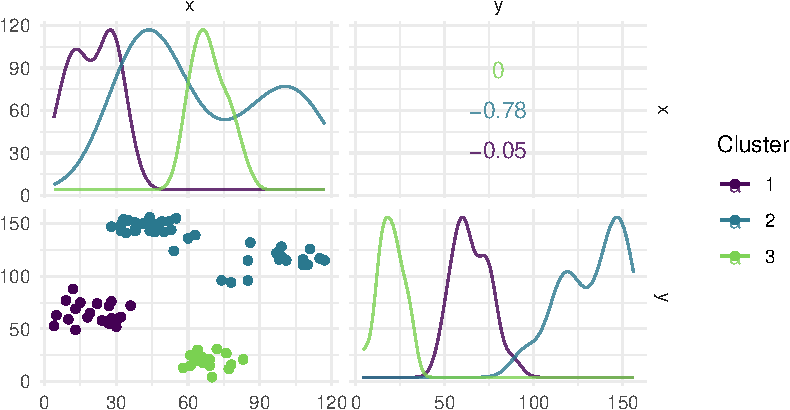
\includegraphics[width=1\textwidth,height=\textheight]{chapters/chapter13/beyond_regression_and_classification_files/figure-pdf/fig-beyond-clust-ruspini-estimated-1.pdf}

}

\caption{\label{fig-beyond-clust-ruspini-estimated}Distribution of the
estimated clusters.}

\end{figure}

While two prediction types are possible, there are some learners where
`prediction' can never make sense, for example in hierarchical
clustering\index{hierarchical clustering}{\marginnote{\begin{footnotesize}Hierarchical
Clustering\end{footnotesize}}}. In hierarchical clustering, the goal is
to build a hierarchy of nested clusters by either splitting large
clusters into smaller ones or merging smaller clusters into bigger ones.
The final result is a tree or dendrogram\index{dendrogram} which can
change if a new data point is added. For consistency,
\texttt{mlr3cluster} offers a \texttt{predict} method for hierarchical
clusters but with a warning:

\begin{Shaded}
\begin{Highlighting}[]
\NormalTok{lrn\_hclust }\OtherTok{=} \FunctionTok{lrn}\NormalTok{(}\StringTok{"clust.hclust"}\NormalTok{, }\AttributeTok{k =} \DecValTok{2}\NormalTok{)}
\NormalTok{lrn\_hclust}\SpecialCharTok{$}\FunctionTok{train}\NormalTok{(tsk\_ruspini)}\SpecialCharTok{$}\FunctionTok{predict}\NormalTok{(tsk\_ruspini)}
\end{Highlighting}
\end{Shaded}

\begin{verbatim}
Warning: Learner 'clust.hclust' doesn't predict on new data and
predictions may not make sense on new data
\end{verbatim}

\begin{verbatim}
<PredictionClust> for 75 observations:
    row_ids partition
          1         1
          2         1
          3         1
---                  
         73         1
         74         1
         75         1
\end{verbatim}

\begin{Shaded}
\begin{Highlighting}[]
\FunctionTok{autoplot}\NormalTok{(lrn\_hclust) }\SpecialCharTok{+} \FunctionTok{theme}\NormalTok{(}\AttributeTok{axis.text =} \FunctionTok{element\_text}\NormalTok{(}\AttributeTok{size =} \FloatTok{5.5}\NormalTok{))}
\end{Highlighting}
\end{Shaded}

\begin{figure}[H]

{\centering 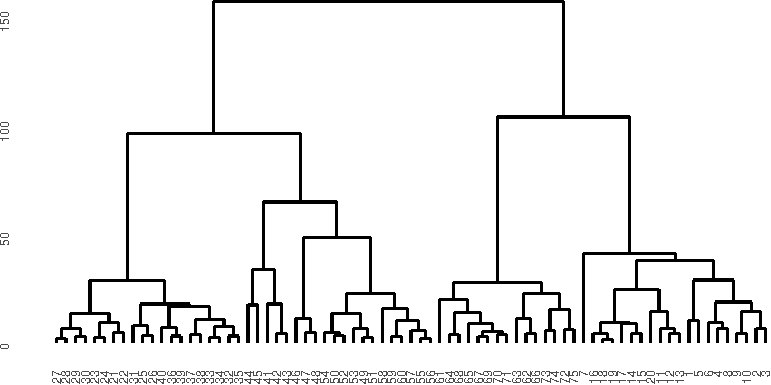
\includegraphics[width=1\textwidth,height=\textheight]{chapters/chapter13/beyond_regression_and_classification_files/figure-pdf/fig-beyond-clust-dend-1.pdf}

}

\caption{\label{fig-beyond-clust-dend}Dendrogram representing
hierarchical clustering of the \texttt{ruspini} dataset. y-axis is
similarity of points such that the lower observations (x-axis) are
connected, the greater their similarity. The top split represents the
separation of the two clusters.}

\end{figure}

In this case, the \texttt{predict} method simply cuts the dendrogram
into the number of clusters specified by \texttt{k} parameter of the
learner.

\hypertarget{measureclust}{%
\subsection{MeasureClust}\label{measureclust}}

As previously discussed, unsupervised tasks do not have ground truth
data to compare to in model evaluation. However, we can still measure
the quality of cluster assignments by quantifying how closely objects
within the same cluster are related (cluster
cohesion\index{cluster cohesion}) as well as how distinct different
clusters are from each other (cluster
separation\index{cluster separation}). There are a few built-in
evaluation metrics available to assess the quality of clustering, which
can be found by searching the
\href{https://mlr3.mlr-org.com/reference/mlr_measures.html}{\texttt{mlr\_measures}}
dictionary.

Two common measures are the within sum of squares (WSS) measure
(\texttt{msr("clust.wss")}) and the silhouette coefficient
(\texttt{msr("clust.silhouette")}). WSS calculates the sum of squared
differences between observations and centroids, which is a
quantification of cluster cohesion (smaller values indicate the clusters
are more compact). The silhouette coefficient quantifies how well each
point belongs to its assigned cluster versus neighboring clusters, where
scores closer to \texttt{1} indicate well clustered and scores closer to
\texttt{-1} indicate poorly clustered. Note that the silhouette measure
in \texttt{mlr3cluster} returns the mean silhouette score across all
observations and when there is only a single cluster, the measure simply
outputs 0.

Putting this together with the above we can now score our cluster
estimation (note we must pass the \texttt{task} to \texttt{\$score}):

\begin{Shaded}
\begin{Highlighting}[]
\NormalTok{measures }\OtherTok{=} \FunctionTok{msrs}\NormalTok{(}\FunctionTok{c}\NormalTok{(}\StringTok{"clust.wss"}\NormalTok{, }\StringTok{"clust.silhouette"}\NormalTok{))}

\NormalTok{prediction}\SpecialCharTok{$}\FunctionTok{score}\NormalTok{(measures, }\AttributeTok{task =}\NormalTok{ tsk\_ruspini)}
\end{Highlighting}
\end{Shaded}

\begin{verbatim}
       clust.wss clust.silhouette 
       5.116e+04        6.414e-01 
\end{verbatim}

The very high WSS and middling mean silhouette coefficient indicate that
our clusters could do with a bit more work.

Often reducing an unsupervised task to a quantitative measure may not be
useful (given no ground truth) and instead visualization (discussed
next) may be a more effective tool for assessing the quality of the
clusters.

\hypertarget{visualization}{%
\subsection{Visualization}\label{visualization}}

As clustering is an unsupervised task, visualization can be essential
not just for `evaluating' models but also for determining if our
learners are performing as expected for our task. This section will look
at visualizations for supporting clustering choices and following that
we will consider plots for evaluating model performance.

\hypertarget{visualizing-clusters}{%
\subsubsection{Visualizing Clusters}\label{visualizing-clusters}}

It is easy to rely on clustering measures to assess the quality of
clustering however this should be done with care as choosing between
models may come down to other decisions such as how clusters are formed.
By example, consider data generated by
\href{https://www.rdocumentation.org/packages/mlbench/topics/mlbench.spirals}{\texttt{mlbench.spirals}},
which results in two individual lines that spiral around each other
(Figure~\ref{fig-beyond-clust-spirals}).

\begin{Shaded}
\begin{Highlighting}[]
\NormalTok{spirals }\OtherTok{=}\NormalTok{ mlbench}\SpecialCharTok{::}\FunctionTok{mlbench.spirals}\NormalTok{(}\AttributeTok{n =} \DecValTok{300}\NormalTok{, }\AttributeTok{sd =} \FloatTok{0.01}\NormalTok{)}
\NormalTok{tsk\_spirals }\OtherTok{=} \FunctionTok{as\_task\_clust}\NormalTok{(}\FunctionTok{as.data.frame}\NormalTok{(spirals}\SpecialCharTok{$}\NormalTok{x))}
\FunctionTok{autoplot}\NormalTok{(tsk\_spirals)}
\end{Highlighting}
\end{Shaded}

\begin{figure}[H]

{\centering 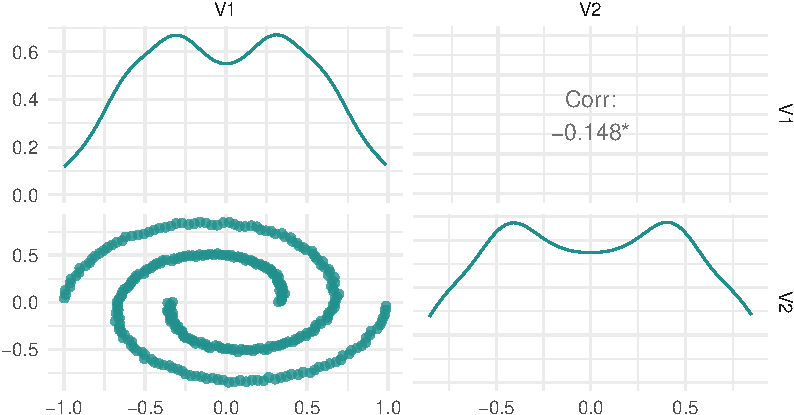
\includegraphics[width=1\textwidth,height=\textheight]{chapters/chapter13/beyond_regression_and_classification_files/figure-pdf/fig-beyond-clust-spirals-1.pdf}

}

\caption{\label{fig-beyond-clust-spirals}Distribution of
\texttt{spirals} data.}

\end{figure}

Now let us see what happens when fit two clustering learners on this
data:

\begin{Shaded}
\begin{Highlighting}[]
\NormalTok{learners }\OtherTok{=} \FunctionTok{list}\NormalTok{(}
  \FunctionTok{lrn}\NormalTok{(}\StringTok{"clust.kmeans"}\NormalTok{),}
  \FunctionTok{lrn}\NormalTok{(}\StringTok{"clust.dbscan"}\NormalTok{, }\AttributeTok{eps =} \FloatTok{0.1}\NormalTok{)}
\NormalTok{)}

\NormalTok{bmr }\OtherTok{=} \FunctionTok{benchmark}\NormalTok{(}\FunctionTok{benchmark\_grid}\NormalTok{(tsk\_spirals, learners, }\FunctionTok{rsmp}\NormalTok{(}\StringTok{"insample"}\NormalTok{)))}
\NormalTok{bmr}\SpecialCharTok{$}\FunctionTok{aggregate}\NormalTok{(}\FunctionTok{msr}\NormalTok{(}\StringTok{"clust.silhouette"}\NormalTok{))[, }\FunctionTok{c}\NormalTok{(}\DecValTok{4}\NormalTok{, }\DecValTok{7}\NormalTok{)]}
\end{Highlighting}
\end{Shaded}

\begin{verbatim}
     learner_id clust.silhouette
1: clust.kmeans          0.37209
2: clust.dbscan          0.02943
\end{verbatim}

We can see that K-means clustering gives us a higher average silhouette
score and so we might conclude that a K-means learner with two centroids
is a better choice than the DBSCAN method. However, now take a look at
the cluster assignment plots in
Figure~\ref{fig-beyond-clust-spirals-pred}
(\texttt{autoplot.PredictionClust} is available but we do not use it
here so we can highlight two particular plots).

\begin{Shaded}
\begin{Highlighting}[]
\FunctionTok{library}\NormalTok{(patchwork)}
\CommentTok{\# get K{-}Means and DBSCAN partitions}
\NormalTok{pred\_kmeans }\OtherTok{=} \FunctionTok{as.factor}\NormalTok{(bmr}\SpecialCharTok{$}\FunctionTok{resample\_result}\NormalTok{(}\DecValTok{1}\NormalTok{)}\SpecialCharTok{$}\FunctionTok{prediction}\NormalTok{()}\SpecialCharTok{$}\NormalTok{partition)}
\NormalTok{pred\_dbscan }\OtherTok{=} \FunctionTok{as.factor}\NormalTok{(bmr}\SpecialCharTok{$}\FunctionTok{resample\_result}\NormalTok{(}\DecValTok{2}\NormalTok{)}\SpecialCharTok{$}\FunctionTok{prediction}\NormalTok{()}\SpecialCharTok{$}\NormalTok{partition)}
\CommentTok{\# plot}
\NormalTok{df\_kmeans }\OtherTok{=} \FunctionTok{cbind}\NormalTok{(tsk\_spirals}\SpecialCharTok{$}\FunctionTok{data}\NormalTok{(), }\AttributeTok{clust =}\NormalTok{ pred\_kmeans)}
\NormalTok{df\_dbscan }\OtherTok{=} \FunctionTok{cbind}\NormalTok{(tsk\_spirals}\SpecialCharTok{$}\FunctionTok{data}\NormalTok{(), }\AttributeTok{clust =}\NormalTok{ pred\_dbscan)}
\NormalTok{map }\OtherTok{=} \FunctionTok{aes}\NormalTok{(}\AttributeTok{x =}\NormalTok{ V1, }\AttributeTok{y =}\NormalTok{ V2, }\AttributeTok{color =}\NormalTok{ clust)}
\NormalTok{p\_kmeans }\OtherTok{=} \FunctionTok{ggplot}\NormalTok{(df\_kmeans, map) }\SpecialCharTok{+} \FunctionTok{ggtitle}\NormalTok{(}\StringTok{"K{-}means"}\NormalTok{)}
\NormalTok{p\_dbscan }\OtherTok{=} \FunctionTok{ggplot}\NormalTok{(df\_dbscan, map) }\SpecialCharTok{+} \FunctionTok{ggtitle}\NormalTok{(}\StringTok{"DBSCAN"}\NormalTok{)}

\NormalTok{p\_kmeans }\SpecialCharTok{+}\NormalTok{ p\_dbscan }\SpecialCharTok{+} \FunctionTok{plot\_layout}\NormalTok{(}\AttributeTok{guides =} \StringTok{"collect"}\NormalTok{) }\SpecialCharTok{\&} \FunctionTok{geom\_point}\NormalTok{() }\SpecialCharTok{\&}
  \FunctionTok{theme\_minimal}\NormalTok{() }\SpecialCharTok{\&}\NormalTok{ ggplot2}\SpecialCharTok{::}\FunctionTok{scale\_colour\_viridis\_d}\NormalTok{(}\AttributeTok{end =} \FloatTok{0.8}\NormalTok{)}
\end{Highlighting}
\end{Shaded}

\begin{figure}[H]

{\centering 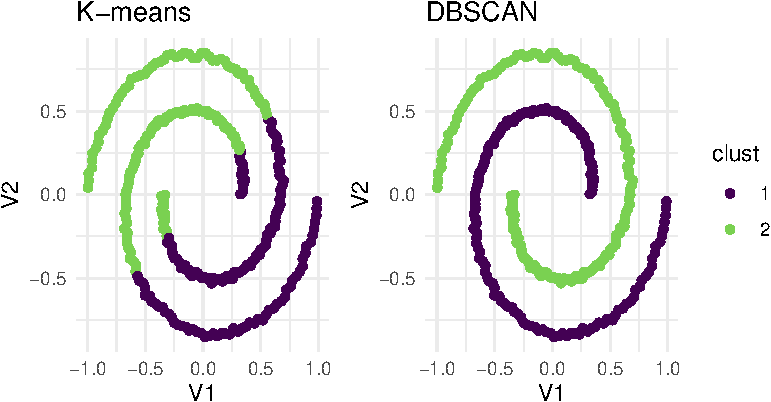
\includegraphics[width=1\textwidth,height=\textheight]{chapters/chapter13/beyond_regression_and_classification_files/figure-pdf/fig-beyond-clust-spirals-pred-1.pdf}

}

\caption{\label{fig-beyond-clust-spirals-pred}Comparing estimated
clusters from \texttt{lrn("clust.kmeans")} and
\texttt{lrn("clust.dbscan")}. Both create two distinct clusters that are
separated in different ways.}

\end{figure}

The two learners arrived at two different results to cleanly separate
clusters -- the K-means algorithm assigned points that are part of the
same line into two different clusters whereas DBSCAN assigned each line
to its own cluster. Which one of these approaches is correct? The answer
is it depends on your specific task and the goal of cluster analysis. If
we had only relied on the silhouette score, then the details of how the
clustering was performed would have been masked and we would have been
unable to decide which method was appropriate for the task.

\hypertarget{pca-and-silhouette-plots}{%
\subsubsection{PCA and Silhouette
Plots}\label{pca-and-silhouette-plots}}

The two most important plots implemented in
\href{https://mlr3viz.mlr-org.com}{\texttt{mlr3viz}}\index{\texttt{mlr3viz}}
to support the evaluation of cluster learners are PCA and silhouette
plots.

Principal components analysis\index{principal components analysis} (PCA)
is a commonly used dimension reduction method in ML to reduce the number
of variables in a dataset or to visualize the most important
`components', which are linear transformations of the dataset features.
Components are considered more important if they have higher variance
(and therefore more predictive power). In the context of clustering, by
plotting observations against the first two components, and then
coloring them by cluster, we could visualize our high-dimensional
dataset and we would expect to see observations in distinct groups.

Since our running example only has two features, PCA does not make sense
to visualize the data. So we will use a task based on the
\texttt{USArrests} dataset instead. By plotting the result of PCA
(Figure~\ref{fig-beyond-clust-usarrests}), we see that our model has
done a good job of separating observations into two clusters along the
first two principal components.

\begin{Shaded}
\begin{Highlighting}[]
\NormalTok{tsk\_usarrests }\OtherTok{=} \FunctionTok{tsk}\NormalTok{(}\StringTok{"usarrests"}\NormalTok{)}
\NormalTok{prediction }\OtherTok{=} \FunctionTok{lrn}\NormalTok{(}\StringTok{"clust.kmeans"}\NormalTok{)}\SpecialCharTok{$}\FunctionTok{train}\NormalTok{(tsk\_usarrests)}\SpecialCharTok{$}
  \FunctionTok{predict}\NormalTok{(tsk\_usarrests)}
\FunctionTok{autoplot}\NormalTok{(prediction, tsk\_usarrests, }\AttributeTok{type =} \StringTok{"pca"}\NormalTok{)}
\end{Highlighting}
\end{Shaded}

\begin{figure}[H]

{\centering 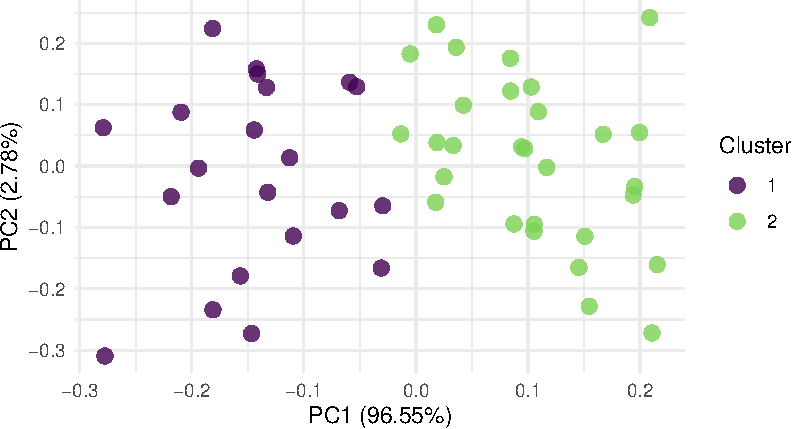
\includegraphics[width=1\textwidth,height=\textheight]{chapters/chapter13/beyond_regression_and_classification_files/figure-pdf/fig-beyond-clust-usarrests-1.pdf}

}

\caption{\label{fig-beyond-clust-usarrests}First two principal
components using PCA on \texttt{tsk("usarrests")}.}

\end{figure}

Silhouette plots visually assess the quality of the estimated clusters
by visualizing if observations in a cluster are well-placed both
individually and as a group. The plots include a dotted line which
visualizes the average silhouette coefficient across all data points and
each data point's silhouette value is represented by a bar colored by
their assigned cluster. In our particular case, the average silhouette
index is 0.59. If the average silhouette value for a given cluster is
below the average silhouette coefficient line then this implies that the
cluster is not well defined.

Continuing with our new example, we find
(Figure~\ref{fig-beyond-clust-sil}) that a lot of observations are
actually below the average line and close to zero, and therefore the
quality of our cluster assignments is not very good, meaning that many
observations are likely assigned to the wrong cluster.

\begin{Shaded}
\begin{Highlighting}[]
\FunctionTok{autoplot}\NormalTok{(prediction, tsk\_usarrests, }\AttributeTok{type =} \StringTok{"sil"}\NormalTok{)}
\end{Highlighting}
\end{Shaded}

\begin{figure}[H]

{\centering 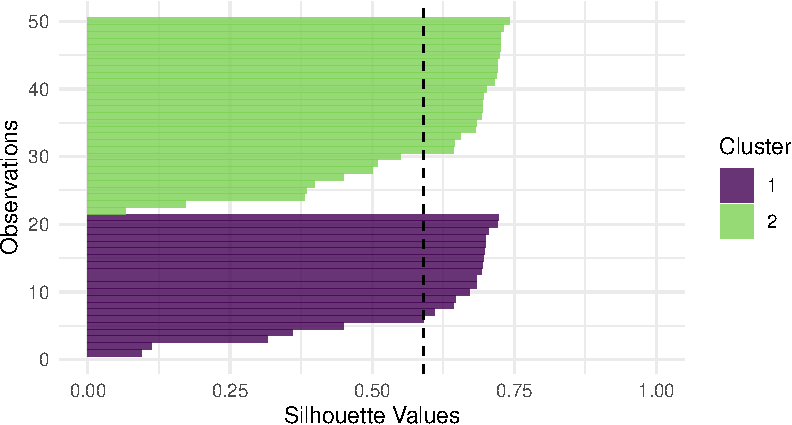
\includegraphics[width=1\textwidth,height=\textheight]{chapters/chapter13/beyond_regression_and_classification_files/figure-pdf/fig-beyond-clust-sil-1.pdf}

}

\caption{\label{fig-beyond-clust-sil}Silhouette plot from predictions
made by \texttt{lrn("clust.kmeans")} on \texttt{tsk("usarrests")}.}

\end{figure}

\hypertarget{sec-cluster-all}{%
\subsection{Putting It All Together}\label{sec-cluster-all}}

Finally, we conduct a small benchmark study using
\texttt{tsk("usarrests")} and a few integrated cluster learners:

\begin{Shaded}
\begin{Highlighting}[]
\NormalTok{tsk\_usarrests }\OtherTok{=} \FunctionTok{tsk}\NormalTok{(}\StringTok{"usarrests"}\NormalTok{)}
\NormalTok{learners }\OtherTok{=} \FunctionTok{list}\NormalTok{(}
  \FunctionTok{lrn}\NormalTok{(}\StringTok{"clust.featureless"}\NormalTok{),}
  \FunctionTok{lrn}\NormalTok{(}\StringTok{"clust.kmeans"}\NormalTok{, }\AttributeTok{centers =}\NormalTok{ 4L),}
  \FunctionTok{lrn}\NormalTok{(}\StringTok{"clust.cmeans"}\NormalTok{, }\AttributeTok{centers =}\NormalTok{ 3L)}
\NormalTok{)}
\NormalTok{measures }\OtherTok{=} \FunctionTok{list}\NormalTok{(}\FunctionTok{msr}\NormalTok{(}\StringTok{"clust.wss"}\NormalTok{), }\FunctionTok{msr}\NormalTok{(}\StringTok{"clust.silhouette"}\NormalTok{))}
\NormalTok{bmr }\OtherTok{=} \FunctionTok{benchmark}\NormalTok{(}\FunctionTok{benchmark\_grid}\NormalTok{(tsk\_usarrests, learners,}
  \FunctionTok{rsmp}\NormalTok{(}\StringTok{"insample"}\NormalTok{)))}
\NormalTok{bmr}\SpecialCharTok{$}\FunctionTok{aggregate}\NormalTok{(measures)[, }\FunctionTok{c}\NormalTok{(}\DecValTok{4}\NormalTok{, }\DecValTok{7}\NormalTok{, }\DecValTok{8}\NormalTok{)]}
\end{Highlighting}
\end{Shaded}

\begin{verbatim}
          learner_id clust.wss clust.silhouette
1: clust.featureless    355808           0.0000
2:      clust.kmeans     34729           0.5012
3:      clust.cmeans     47964           0.5319
\end{verbatim}

The C-means and K-means algorithms are both considerably better than the
featureless baseline but further analysis (and visualizations) would be
required to decide which of those two is suitable for our needs.

\hypertarget{sec-spatiotemporal}{%
\section{Spatial Analysis}\label{sec-spatiotemporal}}

The final task we will discuss in this book is spatial
analysis\index{spatial analysis}. Spatial analysis can be a subset of
any other machine learning task (e.g., regression or classification) and
is defined by the presence of spatial information in a dataset, usually
stored as coordinates that are often named ``x'' and ``y'' or ``lat''
and ``lon'' (for `latitude' and `longitude' respectively.)

Spatial analysis is its own task as spatial data must be handled
carefully due to the complexity of `autocorrelation'. Where
correlation\index{correlation} is defined as a statistical association
\emph{between two} variables,
autocorrelation\index{autocorrelation}{\marginnote{\begin{footnotesize}Autocorrelation\end{footnotesize}}}
is a statistical association \emph{within one} variable. In ML terms, in
a dataset with features and observations, correlation occurs when two or
more features are statistically associated in some way, whereas
autocorrelation occurs when two or more observations are statistically
associated across one feature. Autocorrelation, therefore, violates one
of the fundamental assumptions of ML that all observations in a dataset
are independent, which results in lower confidence about the quality of
a trained machine learning model and the resulting performance estimates
(Hastie, Friedman, and Tibshirani 2001).

Autocorrelation is present in spatial data as there is implicit
information encoded in coordinates, such as whether two observations
(e.g., cities, countries, continents) are close together or far apart.
By example, let us imagine we are predicting the number of cases of a
disease two months after an outbreak in Germany
(Figure~\ref{fig-autocorrelation}). Outbreaks radiate outwards from an
epicenter and therefore countries closer to Germany will have higher
numbers of cases and countries further away will have lower numbers
(Figure~\ref{fig-autocorrelation}, bottom). Thus, looking at the data
spatially shows clear signs of autocorrelation across nearby
observations. Note in this example the autocorrelation is radial but in
practice, this will not always be the case.

\begin{figure}

{\centering 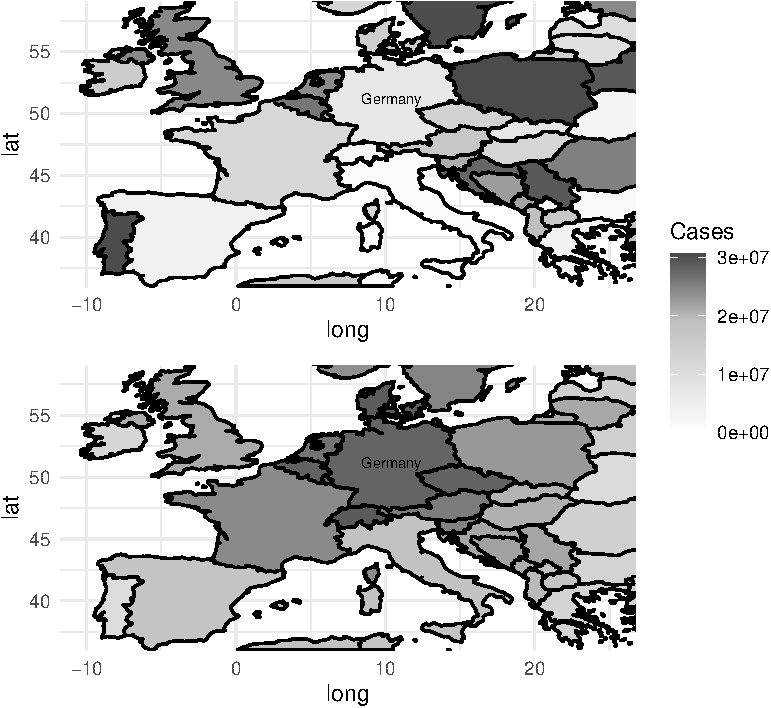
\includegraphics[width=0.6\textwidth,height=0.6\textheight]{chapters/chapter13/beyond_regression_and_classification_files/figure-pdf/fig-autocorrelation-1.pdf}

}

\caption{\label{fig-autocorrelation}Heatmaps where darker countries
indicate higher number of cases and lighter countries indicate lower
number of cases of imaginary Disease X with epicenter in Germany. The
top map imagines a world in which there is no spatial autocorrelation
and the number of cases of a disease is randomly distributed. The bottom
map shows a more accurate world in which the number of cases radiate
outwards from the epicenter (Germany).}

\end{figure}

Unlike other tasks we have looked at in this chapter, there is no
underlying difference between the implemented learners or measures.
Instead, we provide additional resampling methods in
\href{https://mlr3spatiotempcv.mlr-org.com}{\texttt{mlr3spatiotempcv}}\index{\texttt{mlr3spatiotempcv}}
to account for the similarity in the train and test sets during
resampling that originates from spatiotemporal autocorrelation.

Throughout this section we will use the
\href{https://mlr3spatiotempcv.mlr-org.com/reference/ecuador.html}{\texttt{ecuador}}
dataset and task as a working example.

\hypertarget{taskclassifst-and-taskregrst}{%
\subsection{TaskClassifST and
TaskRegrST}\label{taskclassifst-and-taskregrst}}

To make use of spatial resampling methods, we have implemented two
extensions of
\href{https://mlr3.mlr-org.com/reference/TaskClassif.html}{\texttt{TaskClassif}}
and
\href{https://mlr3.mlr-org.com/reference/TaskRegr.html}{\texttt{TaskRegr}}
to accommodate spatial data,
\href{https://mlr3spatiotempcv.mlr-org.com/reference/TaskClassifST.html}{\texttt{TaskClassifST}}
and
\href{https://mlr3spatiotempcv.mlr-org.com/reference/TaskRegrST.html}{\texttt{TaskRegrST}}
respectively. Below we only show classification examples but regression
follows trivially.

\begin{Shaded}
\begin{Highlighting}[]
\FunctionTok{library}\NormalTok{(mlr3spatial)}
\FunctionTok{library}\NormalTok{(mlr3spatiotempcv)}

\CommentTok{\# create task from \textasciigrave{}data.frame\textasciigrave{}}
\NormalTok{tsk\_ecuador }\OtherTok{=} \FunctionTok{as\_task\_classif\_st}\NormalTok{(ecuador, }\AttributeTok{id =} \StringTok{"ecuador\_task"}\NormalTok{,}
  \AttributeTok{target =} \StringTok{"slides"}\NormalTok{, }\AttributeTok{positive =} \StringTok{"TRUE"}\NormalTok{,}
  \AttributeTok{coordinate\_names =} \FunctionTok{c}\NormalTok{(}\StringTok{"x"}\NormalTok{, }\StringTok{"y"}\NormalTok{), }\AttributeTok{crs =} \StringTok{"32717"}\NormalTok{)}

\CommentTok{\# or create task from \textquotesingle{}sf\textquotesingle{} object}
\NormalTok{data\_sf }\OtherTok{=}\NormalTok{ sf}\SpecialCharTok{::}\FunctionTok{st\_as\_sf}\NormalTok{(ecuador, }\AttributeTok{coords =} \FunctionTok{c}\NormalTok{(}\StringTok{"x"}\NormalTok{, }\StringTok{"y"}\NormalTok{), }\AttributeTok{crs =} \StringTok{"32717"}\NormalTok{)}
\NormalTok{tsk\_ecuador }\OtherTok{=} \FunctionTok{as\_task\_classif\_st}\NormalTok{(data\_sf, }\AttributeTok{target =} \StringTok{"slides"}\NormalTok{,}
  \AttributeTok{positive =} \StringTok{"TRUE"}\NormalTok{)}
\NormalTok{tsk\_ecuador}
\end{Highlighting}
\end{Shaded}

\begin{verbatim}
<TaskClassifST:data_sf> (751 x 11)
* Target: slides
* Properties: twoclass
* Features (10):
  - dbl (10): carea, cslope, dem, distdeforest, distroad,
    distslidespast, hcurv, log.carea, slope, vcurv
* Coordinates:
          X       Y
  1: 712882 9560002
  2: 715232 9559582
  3: 715392 9560172
  4: 715042 9559312
  5: 715382 9560142
 ---               
747: 714472 9558482
748: 713142 9560992
749: 713322 9560562
750: 715392 9557932
751: 713802 9560862
\end{verbatim}

Once a task is created, you can train and predict as normal.

\begin{Shaded}
\begin{Highlighting}[]
\FunctionTok{lrn}\NormalTok{(}\StringTok{"classif.rpart"}\NormalTok{)}\SpecialCharTok{$}\FunctionTok{train}\NormalTok{(tsk\_ecuador)}\SpecialCharTok{$}\FunctionTok{predict}\NormalTok{(tsk\_ecuador)}
\end{Highlighting}
\end{Shaded}

\begin{verbatim}
<PredictionClassif> for 751 observations:
    row_ids truth response
          1  TRUE     TRUE
          2  TRUE     TRUE
          3  TRUE     TRUE
---                       
        749 FALSE    FALSE
        750 FALSE    FALSE
        751 FALSE     TRUE
\end{verbatim}

However as discussed above, it is best to use the specialized resampling
methods to achieve bias-reduced estimates of model performance.

\hypertarget{spatiotemp-cv}{%
\subsection{Spatiotemporal Cross-Validation}\label{spatiotemp-cv}}

Before we look at the spatial resampling methods implemented in
\texttt{mlr3spatiotempcv} we will first show what can go wrong if
non-spatial resampling methods are used for spatial data. Below we
benchmark a decision tree on \texttt{tsk("ecuador")} using two different
repeated cross-validation resampling methods, the first (``NSpCV''
(non-spatial cross-validation)) is a non-spatial resampling method from
\texttt{mlr3}, the second (``SpCV'' (spatial cross-validation)) is from
\texttt{mlr3spatiotempcv} and is optimized for spatial data. The example
highlights how ``NSpCV'' makes it appear as if the decision tree is
performing better than it is with considerably higher estimated
performance, however, this is an overconfident prediction due to the
autocorrelation in the data.

\begin{Shaded}
\begin{Highlighting}[]
\NormalTok{lrn\_rpart }\OtherTok{=} \FunctionTok{lrn}\NormalTok{(}\StringTok{"classif.rpart"}\NormalTok{, }\AttributeTok{predict\_type =} \StringTok{"prob"}\NormalTok{)}
\NormalTok{rsmp\_nsp }\OtherTok{=} \FunctionTok{rsmp}\NormalTok{(}\StringTok{"repeated\_cv"}\NormalTok{, }\AttributeTok{folds =} \DecValTok{3}\NormalTok{, }\AttributeTok{repeats =} \DecValTok{2}\NormalTok{, }\AttributeTok{id =} \StringTok{"NSpCV"}\NormalTok{)}
\NormalTok{rsmp\_sp }\OtherTok{=} \FunctionTok{rsmp}\NormalTok{(}\StringTok{"repeated\_spcv\_coords"}\NormalTok{, }\AttributeTok{folds =} \DecValTok{3}\NormalTok{, }\AttributeTok{repeats =} \DecValTok{2}\NormalTok{,}
  \AttributeTok{id =} \StringTok{"SpCV"}\NormalTok{)}

\NormalTok{design }\OtherTok{=} \FunctionTok{benchmark\_grid}\NormalTok{(tsk\_ecuador, lrn\_rpart, }\FunctionTok{c}\NormalTok{(rsmp\_nsp, rsmp\_sp))}
\NormalTok{bmr }\OtherTok{=} \FunctionTok{benchmark}\NormalTok{(design)}
\NormalTok{bmr}\SpecialCharTok{$}\FunctionTok{aggregate}\NormalTok{(}\FunctionTok{msr}\NormalTok{(}\StringTok{"classif.acc"}\NormalTok{))[, }\FunctionTok{c}\NormalTok{(}\DecValTok{5}\NormalTok{, }\DecValTok{7}\NormalTok{)]}
\end{Highlighting}
\end{Shaded}

\begin{verbatim}
   resampling_id classif.acc
1:         NSpCV      0.6718
2:          SpCV      0.5842
\end{verbatim}

In the above example, applying non-spatial resampling results in train
and test sets that are very similar due to the underlying spatial
autocorrelation. Hence there is little difference from testing a model
on the same data it was trained on, which should be avoided for an
honest performance result (see Chapter~\ref{sec-basics}). In contrast,
the spatial method has accommodated autocorrelation and the test data is
less correlated (though some association will remain) with the training
data. Visually this can be seen using
\href{https://mlr3spatiotempcv.mlr-org.com/reference/autoplot.html}{\texttt{autoplot()}}
methods. In Figure~\ref{fig-sprsmp} we visualize how the task is
partitioned according to the spatial resampling method
(Figure~\ref{fig-sprsmp}, left) and non-spatial resampling method
(Figure~\ref{fig-sprsmp}, right). There is a clear separation in space
for the respective partitions when using the spatial resampling whereas
the train and test splits overlap a lot (and are therefore more
correlated) using the non-spatial method.

\begin{Shaded}
\begin{Highlighting}[]
\FunctionTok{library}\NormalTok{(patchwork)}

\NormalTok{(}\FunctionTok{autoplot}\NormalTok{(rsmp\_sp, tsk\_ecuador, }\AttributeTok{fold\_id =} \DecValTok{1}\NormalTok{, }\AttributeTok{size =} \FloatTok{0.7}\NormalTok{) }\SpecialCharTok{+}
  \FunctionTok{ggtitle}\NormalTok{(}\StringTok{"Spatial Resampling"}\NormalTok{) }\SpecialCharTok{+}
  \FunctionTok{autoplot}\NormalTok{(rsmp\_nsp, tsk\_ecuador, }\AttributeTok{fold\_id =} \DecValTok{1}\NormalTok{, }\AttributeTok{size =} \FloatTok{0.7}\NormalTok{) }\SpecialCharTok{+}
  \FunctionTok{ggtitle}\NormalTok{(}\StringTok{"Non{-}spatial Resampling"}\NormalTok{)) }\SpecialCharTok{+}
  \FunctionTok{plot\_layout}\NormalTok{(}\AttributeTok{guides =} \StringTok{"collect"}\NormalTok{) }\SpecialCharTok{\&}
  \FunctionTok{theme\_minimal}\NormalTok{() }\SpecialCharTok{\&}
  \FunctionTok{theme}\NormalTok{(}\AttributeTok{axis.text =} \FunctionTok{element\_text}\NormalTok{(}\AttributeTok{size =} \DecValTok{4}\NormalTok{), }\AttributeTok{legend.position =} \StringTok{"bottom"}\NormalTok{)}
\end{Highlighting}
\end{Shaded}

\begin{figure}[H]

{\centering 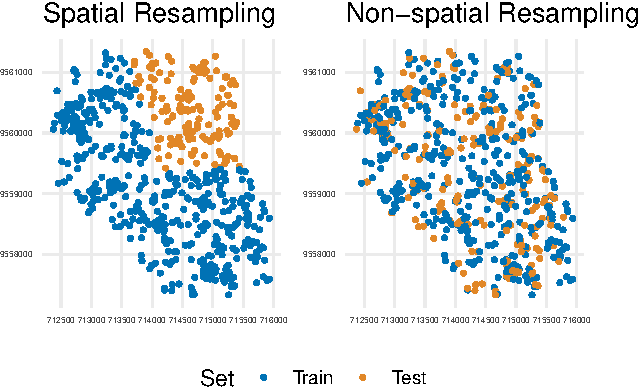
\includegraphics[width=1\textwidth,height=\textheight]{chapters/chapter13/beyond_regression_and_classification_files/figure-pdf/fig-sprsmp-1.pdf}

}

\caption{\label{fig-sprsmp}Scatterplots show separation of train (blue)
and test (orange) data for the first fold of the first repetition of the
cross-validation. Left is spatial resampling where train and test data
are clearly separated. Right is non-spatial resampling where there is
overlap in train and test data.}

\end{figure}

Now we have seen why spatial resampling matters we can take a look at
what methods are available in \texttt{mlr3spatiotempcv}. The resampling
methods we have added can be categorized into:

\begin{itemize}
\tightlist
\item
  Blocking -- Create rectangular blocks in 2D or 3D space
\item
  Buffering -- Create buffering zones to remove observations between
  train and test sets
\item
  Spatiotemporal clustering -- Clusters based on coordinates (and/or
  time points)
\item
  Feature space clustering -- Clusters based on feature space and not
  necessarily spatiotemporal
\item
  Custom (partitioning) -- Grouped by factor variables
\end{itemize}

The choice of method may depend on specific characteristics of the
dataset and there is no easy rule to pick one method over another, full
details of different methods can be found in Schratz et al. (2021) --
the paper deliberately avoids recommending one method over another as
the `optimal' choice is highly dependent on the predictive task,
autocorrelation in the data, and the spatial structure of the sampling
design. The documentation for each of the implemented methods includes
details of each method as well as references to original publications.

\begin{tcolorbox}[enhanced jigsaw, opacitybacktitle=0.6, rightrule=.15mm, opacityback=0, arc=.35mm, breakable, titlerule=0mm, colframe=quarto-callout-tip-color-frame, coltitle=black, bottomrule=.15mm, toprule=.15mm, colback=white, colbacktitle=quarto-callout-tip-color!10!white, bottomtitle=1mm, toptitle=1mm, title=\textcolor{quarto-callout-tip-color}{\faLightbulb}\hspace{0.5em}{Spatio\emph{temporal} Resampling}, leftrule=.75mm, left=2mm]

We have focused on spatial analysis but referred to ``spatiotemporal''
and ``spatiotemp''. The spatial-only resampling methods discussed in
this section can be extended to temporal analysis (or spatial and
temporal analysis combined) by setting the \texttt{"time"}
\texttt{col\_role} in the task (Section~\ref{sec-row-col-roles}) -- this
is an advanced topic that may be added in future editions of this book.
See the \texttt{mlr3spatiotempcv} visualization vignette at
\url{https://mlr3spatiotempcv.mlr-org.com/articles/spatiotemp-viz.html}
for specific details about 3D spatiotemporal visualization.

\end{tcolorbox}

\hypertarget{sec-spatial-prediction}{%
\subsection{Spatial Prediction}\label{sec-spatial-prediction}}

Until now we have looked at resampling to accommodate spatiotemporal
\emph{features}, but what if you want to make spatiotemporal
\emph{predictions}? In this case, the goal is to make classification or
regression predictions at the pixel level, i.e., for an area, defined by
the geometric resolution, of a raster image.

To enable these predictions we have created a new function,
\href{https://mlr3spatial.mlr-org.com/reference/predict_spatial.html}{\texttt{predict\_spatial()}},
to allow spatial predictions using any of the following spatial data
classes:

\begin{itemize}
\tightlist
\item
  \texttt{stars} (from package
  \href{https://cran.r-project.org/package=stars}{\texttt{stars}})
\item
  \texttt{SpatRaster} (from package
  \href{https://cran.r-project.org/package=terra}{\texttt{terra}})
\item
  \texttt{RasterLayer} (from package
  \href{https://cran.r-project.org/package=raster}{\texttt{raster}})
\item
  \texttt{RasterStack} (from package
  \href{https://cran.r-project.org/package=raster}{\texttt{raster}})
\end{itemize}

In the example below we load the \texttt{leipzig\_points} dataset for
training and coerce this to a spatiotemporal task with
\href{https://mlr3spatiotempcv.mlr-org.com/reference/as_task_classif_st.html}{\texttt{as\_task\_classif\_st}},
and we load the \texttt{leipzig\_raster} raster. Both files are included
as example data in
\href{https://mlr3spatial.mlr-org.com}{\texttt{mlr3spatial}}\index{\texttt{mlr3spatial}}.

\begin{Shaded}
\begin{Highlighting}[]
\FunctionTok{library}\NormalTok{(mlr3spatial)}
\FunctionTok{library}\NormalTok{(sf)}
\FunctionTok{library}\NormalTok{(terra, }\AttributeTok{exclude =} \StringTok{"resample"}\NormalTok{)}

\CommentTok{\# load sample points}
\NormalTok{leipzig\_vector }\OtherTok{=}\NormalTok{ sf}\SpecialCharTok{::}\FunctionTok{read\_sf}\NormalTok{(}\FunctionTok{system.file}\NormalTok{(}\StringTok{"extdata"}\NormalTok{,}
  \StringTok{"leipzig\_points.gpkg"}\NormalTok{, }\AttributeTok{package =} \StringTok{"mlr3spatial"}\NormalTok{),}
  \AttributeTok{stringsAsFactors =} \ConstantTok{TRUE}\NormalTok{)}
\CommentTok{\# create training data}
\NormalTok{tsk\_leipzig }\OtherTok{=} \FunctionTok{as\_task\_classif\_st}\NormalTok{(leipzig\_vector, }\AttributeTok{target =} \StringTok{"land\_cover"}\NormalTok{)}

\CommentTok{\# load raster image}
\NormalTok{leipzig\_raster }\OtherTok{=}\NormalTok{ terra}\SpecialCharTok{::}\FunctionTok{rast}\NormalTok{(}\FunctionTok{system.file}\NormalTok{(}\StringTok{"extdata"}\NormalTok{, }\StringTok{"leipzig\_raster.tif"}\NormalTok{,}
  \AttributeTok{package =} \StringTok{"mlr3spatial"}\NormalTok{))}
\end{Highlighting}
\end{Shaded}

Now we can continue as normal to train and predict with a classification
learner, in this case, a random forest.

\begin{Shaded}
\begin{Highlighting}[]
\NormalTok{lrn\_ranger }\OtherTok{=} \FunctionTok{lrn}\NormalTok{(}\StringTok{"classif.ranger"}\NormalTok{)}\SpecialCharTok{$}\FunctionTok{train}\NormalTok{(tsk\_leipzig)}
\NormalTok{prediction }\OtherTok{=} \FunctionTok{predict\_spatial}\NormalTok{(leipzig\_raster, lrn\_ranger,}
  \AttributeTok{format =} \StringTok{"terra"}\NormalTok{)}
\NormalTok{prediction}
\end{Highlighting}
\end{Shaded}

\begin{verbatim}
class       : SpatRaster 
dimensions  : 206, 154, 1  (nrow, ncol, nlyr)
resolution  : 10, 10  (x, y)
extent      : 731810, 733350, 5692030, 5694090  (xmin, xmax, ymin, ymax)
coord. ref. : WGS 84 / UTM zone 32N (EPSG:32632) 
source      : file3aaf41170ae0.tif 
categories  : categories 
name        : land_cover 
min value   :     forest 
max value   :      water 
\end{verbatim}

In this example, we specified the creation of a \texttt{terra} object,
which can be visualized with in-built plotting methods.

\begin{Shaded}
\begin{Highlighting}[]
\FunctionTok{plot}\NormalTok{(prediction, }\AttributeTok{col =} \FunctionTok{c}\NormalTok{(}\StringTok{"\#440154FF"}\NormalTok{, }\StringTok{"\#443A83FF"}\NormalTok{, }\StringTok{"\#31688EFF"}\NormalTok{,}
  \StringTok{"\#21908CFF"}\NormalTok{, }\StringTok{"\#35B779FF"}\NormalTok{, }\StringTok{"\#8FD744FF"}\NormalTok{, }\StringTok{"\#FDE725FF"}\NormalTok{))}
\end{Highlighting}
\end{Shaded}

\begin{figure}[H]

{\centering 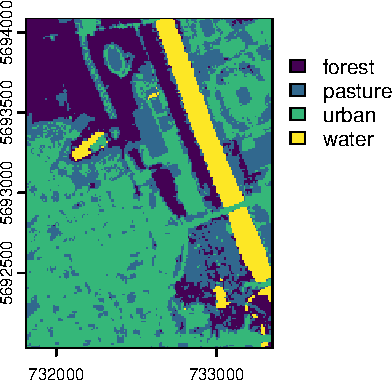
\includegraphics[width=0.5\textwidth,height=0.5\textheight]{chapters/chapter13/beyond_regression_and_classification_files/figure-pdf/fig-beyond-raster-1.pdf}

}

\caption{\label{fig-beyond-raster}Spatial predictions for forest
(purple), pasture (blue), urban (green), and water (yellow) categories.}

\end{figure}

\hypertarget{conclusion-10}{%
\section{Conclusion}\label{conclusion-10}}

In this chapter, we explored going beyond regression and classification
to see how classes in \texttt{mlr3} can be used to implement other ML
tasks. Cost-sensitive classification extends the `normal' classification
setting by assuming that costs associated with false
negatives\index{false negative} and false
positives\index{false positive} are unequal. Running cost-sensitive
classification experiments is possible using only features in
\texttt{mlr3}. Survival analysis, available in
\href{https://mlr3proba.mlr-org.com}{\texttt{mlr3proba}}\index{\texttt{mlr3proba}},
can be thought of as a regression problem when the outcome may be
censored, which means it may never be observed within a given time
frame. The final task in \texttt{mlr3proba} is density estimation, the
unsupervised task concerned with estimating univariate probability
distributions. Using
\href{https://mlr3cluster.mlr-org.com}{\texttt{mlr3cluster}}\index{\texttt{mlr3cluster}},
you can perform cluster analysis on observations, which involves
grouping observations according to similarities in their variables.
Finally, with
\href{https://mlr3spatial.mlr-org.com}{\texttt{mlr3spatial}}\index{\texttt{mlr3spatial}}
and
\href{https://mlr3spatiotempcv.mlr-org.com}{\texttt{mlr3spatiotempcv}}\index{\texttt{mlr3spatiotempcv}},
it is possible to perform spatial analysis to make predictions using
coordinates as features and to make spatial predictions. The
\texttt{mlr3} interface is highly extensible, which means future ML
tasks can (and will) be added to our universe and we will add these to
this chapter of the book in future editions.

\hypertarget{tbl-beyond-api}{}
\begin{longtable}[]{@{}
  >{\raggedright\arraybackslash}p{(\columnwidth - 4\tabcolsep) * \real{0.5000}}
  >{\raggedright\arraybackslash}p{(\columnwidth - 4\tabcolsep) * \real{0.3000}}
  >{\raggedright\arraybackslash}p{(\columnwidth - 4\tabcolsep) * \real{0.2000}}@{}}
\caption{\label{tbl-beyond-api}Important classes and functions covered
in this chapter with underlying class (if applicable), class constructor
or function, and important class fields and methods (if
applicable).}\tabularnewline
\toprule\noalign{}
\begin{minipage}[b]{\linewidth}\raggedright
Class
\end{minipage} & \begin{minipage}[b]{\linewidth}\raggedright
Constructor/Function
\end{minipage} & \begin{minipage}[b]{\linewidth}\raggedright
Fields/Methods
\end{minipage} \\
\midrule\noalign{}
\endfirsthead
\toprule\noalign{}
\begin{minipage}[b]{\linewidth}\raggedright
Class
\end{minipage} & \begin{minipage}[b]{\linewidth}\raggedright
Constructor/Function
\end{minipage} & \begin{minipage}[b]{\linewidth}\raggedright
Fields/Methods
\end{minipage} \\
\midrule\noalign{}
\endhead
\bottomrule\noalign{}
\endlastfoot
\href{https://mlr3.mlr-org.com/reference/MeasureClassifCosts.html}{\texttt{MeasureClassifCosts}}
& \texttt{msr("classif.costs")} & - \\
\href{https://mlr3pipelines.mlr-org.com/reference/PipeOpTuneThreshold.html}{\texttt{PipeOpTuneThreshold}}
& \texttt{po("tunethreshold")} & - \\
\href{https://mlr3proba.mlr-org.com/reference/TaskSurv.html}{\texttt{TaskSurv}}
&
\href{https://mlr3proba.mlr-org.com/reference/as_task_surv.html}{\texttt{as\_task\_surv()}}
& \texttt{\$data()} \\
\href{https://mlr3proba.mlr-org.com/reference/PipeOpDistrCompositor.html}{\texttt{PipeOpDistrCompositor}}
& \texttt{po("distrcompose")} & - \\
\href{https://mlr3proba.mlr-org.com/reference/TaskDens.html}{\texttt{TaskDens}}
&
\href{https://mlr3proba.mlr-org.com/reference/as_task_dens.html}{\texttt{as\_task\_dens()}}
& \texttt{\$data()} \\
\href{https://mlr3cluster.mlr-org.com/reference/TaskClust.html}{\texttt{TaskClust}}
&
\href{https://mlr3cluster.mlr-org.com/reference/as_task_clust.html}{\texttt{as\_task\_clust()}}
& \texttt{\$data()} \\
\href{https://mlr3spatiotempcv.mlr-org.com/reference/TaskClassifST.html}{\texttt{TaskClassifST}}
&
\href{https://mlr3spatiotempcv.mlr-org.com/reference/as_task_classif_st.html}{\texttt{as\_task\_classif\_st()}}
& \texttt{\$data()} \\
- &
\href{https://mlr3spatiotempcv.mlr-org.com/reference/predict_spatial.html}{\texttt{predict\_spatial()}}
& \\
\end{longtable}

\hypertarget{exercises-11}{%
\section{Exercises}\label{exercises-11}}

\begin{enumerate}
\def\labelenumi{\arabic{enumi}.}
\tightlist
\item
  Run a benchmark experiment on \texttt{tsk("german\_credit")} with
  \texttt{lrn("classif.featureless")}, \texttt{lrn("classif.log\_reg")},
  and \texttt{lrn("classif.ranger")}. Tune the prediction thresholds of
  all learners by encapsulating them in a \texttt{po("learner\_cv")}
  (with two-fold CV), followed by a \texttt{po("tunethreshold")}. Use
  \texttt{msr("classif.costs",\ costs\ =\ costs)}, where the
  \texttt{costs} matrix is as follows: true positive is \texttt{-10},
  true negative is \texttt{-1}, false positive is \texttt{2}, and false
  negative is \texttt{3}. Use this measure in
  \texttt{po("tunethreshold")} and when evaluating your benchmark
  experiment.
\item
  Train and test a survival forest using \texttt{lrn("surv.rfsrc")}
  (from \texttt{mlr3extralearners}). Run this experiment using
  \texttt{tsk("rats")} and \texttt{partition()}. Evaluate your model
  with the RCLL measure.
\item
  Estimate the density of the ``precip'' task from the
  \texttt{mlr3proba} package using \texttt{lrn("dens.hist")}, evaluate
  your estimation with the logloss measure. As a stretch goal, look into
  the documentation of \texttt{distr6} to learn how to analyse your
  estimated distribution further.
\item
  Run a benchmark clustering experiment on the ``wine'' dataset without
  a label column. Compare the performance of k-means learner with
  \texttt{k} equal to \texttt{2}, \texttt{3} and \texttt{4} using the
  silhouette measure and the insample resampling technique. What value
  of \texttt{k} would you choose based on the silhouette scores?
\end{enumerate}
